\documentclass[11pt]{article}
\usepackage[a4paper, portrait, margin=1.1811in]{geometry}
\usepackage[english]{babel}
\usepackage[utf8]{inputenc}
\usepackage[T1]{fontenc}
\usepackage{lmodern}
%\usepackage{helvet}
%\renewcommand{\familydefault}{\sfdefault}
\usepackage{etoolbox}
\usepackage{graphicx}
\usepackage{titlesec}
\usepackage{caption}
\usepackage{booktabs}
\usepackage{xcolor} 
\usepackage{breakcites}
\usepackage{caption}
\usepackage{float}
\captionsetup[figure]{name=Figure}
\usepackage{setspace}
\graphicspath{ {./images/} }
\usepackage{scrextend}
\usepackage{subfigure}
\usepackage{tabularx}
\usepackage{fancyhdr}
\usepackage{graphicx}
\usepackage{acronym}
\usepackage{comment}

% Math packs
\usepackage{amsmath}
\usepackage{amssymb}

% footnotes
\usepackage[hang, flushmargin]{footmisc}
\usepackage[colorlinks=true, citecolor=cyan]{hyperref}
\usepackage{footnotebackref}

\newcounter{lemma}
\newtheorem{lemma}{Lemma}
\newcounter{theorem}
\newtheorem{theorem}{Theorem}

%\pagestyle{plain}
\makeatletter
\patchcmd{\@maketitle}{\LARGE \@title}{\fontsize{16}{19.2}\selectfont\@title}{}{}
\makeatother

\usepackage{authblk}
\newcolumntype{C}[1]{>{\centering\let\newline\\\arraybackslash\hspace{0pt}}m{#1}}
\renewcommand\Authfont{\fontsize{12}{10.8}\selectfont}
\renewcommand\Affilfont{\fontsize{12}{10.8}\selectfont}
\renewcommand*{\Authsep}{, }
\renewcommand*{\Authand}{, }
\renewcommand*{\Authands}{, }
\newcommand{\rvec}{\mathrm {\mathbf {r}}} 
\renewcommand{\thetable}{S\arabic{table}}
\setlength{\affilsep}{2em}  
\newsavebox\affbox
\author[a]{\textbf{Jörg Breitung}}
\author[b]{\textbf{Lennart Bolwin}}
\author[b]{\textbf{Justus Töns}}
\affil[a]{University of Cologne, Chair of Statistics and Econometrics}
\affil[b]{University of Cologne, Chair of Statistics and Econometrics \newline
	Supervised by Prof. Jörg Breitung
}


\titlespacing\section{0pt}{12pt plus 4pt minus 2pt}{0pt plus 2pt minus 2pt}
\titlespacing\subsection{12pt}{12pt plus 4pt minus 2pt}{0pt plus 2pt minus 2pt}
\titlespacing\subsubsection{12pt}{12pt plus 4pt minus 2pt}{0pt plus 2pt minus 2pt}


\titleformat{\section}{\normalfont\fontsize{14}{15}\bfseries}{\thesection.}{1em}{}
\titleformat{\subsection}{\normalfont\fontsize{12}{15}\bfseries}{\thesubsection.}{1em}{}
\titleformat{\subsubsection}{\normalfont\fontsize{12}{15}\bfseries}{\thesubsubsection.}{1em}{}

\titleformat{\author}{\normalfont\fontsize{10}{15}\bfseries}{\thesection}{1em}{}

\title{\textbf{\huge Combining Synthetic Controls and VARs:}\\
	On the Estimation of Causal Effects in Time Series Data}
\date{}    

\begin{document}
	\onehalfspacing
	\pagestyle{headings}	
	\newpage
	\setcounter{page}{1}
	\renewcommand{\thepage}{\arabic{page}}
	
	
	
	\captionsetup[figure]{labelfont={bf},labelformat={default},labelsep=period,name={Figure }}	\captionsetup[table]{labelfont={bf},labelformat={default},labelsep=period,name={Table }}
	\setlength{\parskip}{0.5em}
	
	\maketitle
	
	\noindent\rule{15cm}{0.5pt}
	\begin{abstract}
		We argue that applications of \ac{SC} are faced with a self-selection problem. That is, the method is primarily applied to non-complex data structures that are straightforward to forecast, given the availability of donors in the post-treatment period. Using simulation  studies, we show that the high interpretability of \ac{SC} comes at the cost of poor predictions and forecasts, which are especially pronounced if the data generating process contains a time series structure. To address this issue, we introduce the intricacy-statistics that informs the applied researcher whether or not the data at hand exceeds a level of time series structure that \ac{SC} can handle. If the case, more flexible methodologies that combine the strengths of \ac{SC} and conventional time series techniques promise more accurate predictions and forecasts. Hence we introduce the new \ac{VARSC} estimator, that takes in account both the time series structure and the availability of donors. In order to implement these ideas, we introduce the R-package varsc that provides ready-to-use functions to compute the intricacy-statistics and, based on the magnitude of the statistics, the functionalities to estimate either the \ac{SC} or the \ac{VARSC} model. To probe the performance of our methodology outside the experimental setting, we apply it to three existing applications of \ac{SC}: Specifically, we show that our proposed model performs equally well like the SC-method. The result is striking because in contrast to the \ac{SC}-model, our models gets along without the informational contend of potential covariates. \\ \\
		
		\textbf{\textit{Keywords}}: \textit{Synthetic Control; Causality; VAR}
	\end{abstract}
	\noindent\rule{15cm}{0.4pt}
	
	
	% einzelne Abschnitte
	\newpage
	\doublespacing
	\section*{List of Acronyms}
\begin{acronym}
	\acro{ADH}{Abadie, Diamond, and Hainmueller}
	\acro{ARDL}{Autoregressive Distributed Lag}
	\acro{GDP}{Gross Domestic Product}
	\acro{DGP}{Data Generating Process}
	\acro{iid}{independent and identically distributed}
	\acro{MSFE}{Mean Squared Forecast Error}
	\acro{MSPE}{Mean Squared Prediction Error}
	\acro{OLS}{Ordinary Least Squares}
	\acro{PC}{Principal Components}
	\acro{REGSC}{Regularized Synthetic Controls}
	\acro{RSS}{Residual Sum of Squares}
	\acro{SC}{Synthetic Control}
	\acro{USA}{United States of America}
	\acro{VAR}{Vector Autoregression}
	\acro{VARSC}{Vector Autoregressive Synthetic Control}
\end{acronym}
	\newpage
	\tableofcontents
	\newpage
	\listoffigures
	\newpage
	\section{Introduction}

\textcolor{magenta}{\textbf{This is work in progress}}

\ac{SC} method is combined with \ac{VAR}. Method was introduced by \ac{ADH}. Paper strcuture could be similar to the one by \cite{doudchenko:2016}
	\newpage	
	\section{Literature Review 2-3 pages}

\textcolor{magenta}{\textbf{What must be clear by now
		\begin{itemize}
			\item ...
		\end{itemize}}}

\subsection{Synthetic Control}
The \ac{SC} method was developed by Alberto Abadie and colleagues in a series of influential papers (\cite{abadie:2003}, \cite{abadie:2010}, \cite{abadie:2015}). The method is designed to estimate the causal effect of a treatment in a setting with a single treatment unit and a number of potential control units. Pre- and post-treatment data are observed for the treatment and control units for the outcome of interest as well as for a set of covariates. The \ac{SC}-procedure combines aspects of the matching and difference-in-difference literature and can therefore be interpreted as a relative of the causal inference literature introduced by \cite{rubin:1974}. Similar to many other microeconometric methods, the objective is to distinguish causation from correlation and to assess the magnitude and significance of treatments in observational case studies.
\\
In their canonical 2003 article, Abadie and Gardeazabal evaluate the causal economic effects of conflict using terrorist conflicts in the Basque Country as a comparative case study.  In their specific application example, they find that terrorist conflicts caused the per capita \ac{GDP} of the treatment unit (Basque Country) to decline by about 10\% relative to the synthesized control unit. 

\textbf{some more words on other findis and things they did}
The next appropriate setting for an application of the \ac{SC} method was the introduction of a large-scale tobacco control program implemented in the state of California in the \ac{USA} in 1988. 

 


\subsection{Overview}
\cite{abadie:2021a} read.\\
\cite{athey:2016} read.

\subsection{Application}
\cite{born:2019} read. \\
\cite{cho:2020} read.\\
\cite{cunningham:2021} read.\\
\cite{funke:2020} read.

\subsection{Methodological Background}
\cite{abadie:2011} read.\\
\cite{abadie:2006} not read.\\
\cite{abadie:2002} not read.\\
\cite{doudchenko:2016} read. \\
\cite{ferman:2021} read.\\
\cite{frangakis:2002} not read.\\
\cite{rosenbaum:1983} not read \\
\cite{rubin:1974} not read.

\subsection{Extensions/ Developments}
\cite{abadie:2019} read.\\
\cite{amjad:2018} read.\\
\cite{benmichael:2021a} read.\\
\cite{benmichael:2021b} not read. \\
\cite{kellog:2021} not read. \\
\cite{kuosmanen:2021} not read.\\
\cite{muhlbach:2019} read.

\textit{Developments}\\
\cite{arkhangelsky:2021} not read\\
\cite{athey:2017} not read.\\
\cite{brodersen:2015} read. \\
\cite{brzeski:2015} read. \\
\cite{hartford:2017} read.

\subsection{Testing}
\cite{andrews:2003} not read. \\
\cite{cattaneo:2021} not read. \\
\cite{chernozhukov:2019} not read.\\
\cite{chernozhukov:2021} not read. \\
\cite{firpo:2018} not read. \\
\cite{hahn:2017} read.

\subsection{Time Series Econometrics}
\cite{martin:2012} read.\\
\cite{harvey:2020} read.\\
\cite{breitung:2021} partially read.


	\newpage
	\section{Theory}

\textcolor{magenta}{\textbf{What must be clear by now
	 \begin{itemize}
	 	\item Consider case without covariates
	 	\item Make clear that SC is a weighted average of the donors
	 	\item ...
	 \end{itemize}}}

In this chapter, we propose an alternative \ac{SC}-estimator to assess the magnitude of treatment effects in observational settings. To establish a general basis, let us first describe the contextual environment of the estimation. Similar to the setting as introduced by \ac{ADH}, we consider a framework with $J+1$ panel units indexed by $j = 0,1, ..., J$ that are observed over a time horizon of $T$ periods. Without loss of generality, assume that unit $j = 0$, is exposed to the treatment at period $t = T_0$ with $1 < T_0 < T$ and that there are no treatment anticipation and contamination. To contextualize these assumptions, \cite{abadie:2010} argue that in the presence of anticipation effects, $T_0$ could be shifted back in time until the assumptions seems plausible. If panel units in the donor pool\footnote{To ensure direct comparability with the \ac{SC} literature, we adopt most of the commonly used terms. For example, control group units are labeled as 'donors'.} are affected by the treatment (contamination) as it is likely in Brexit-application, those units could be removed from the sample prior to the estimation. Our goal is to evaluate the causal effect of the treatment, the specific functional form of which has yet to be specified.

The following theoretical argumentation is structured as follows: To have a common denominator, we first describe the canonical estimation procedure as proposed by \ac{ADH}. Next we build intuition by considering a very simple static scenario with only two donor units and one treatment unit. We then generalize this idea to the case with many potential donors. The main difference to the setting of \ac{ADH} is that we remove some of the weight constraints and that we analyze a situation without covariates. The former distinction guides us to the field of regularization in order to prevent our method from overfitting. The latter drastically reduces the data requirements but causes our algorithm to estimate the counterfactual with a significantly smaller information set. This fact leads us to our main contribution: The integration of  multivariate time series approaches into the \ac{SC}-algorithm. 

\subsection{\ac{ADH} Case}
We start by presenting the \ac{SC}-method in its original form as introduced \ac{ADH}. Besides introducing the general estimation technique, we also want to elaborate on the proposed hypothesis testing procedure of \ac{ADH}. For the sake of comparability and due to its notational and inhat clarity, we borrow the employed notation. 

\textit{Setup} \\
The estimation task can be constituted by the potential outcome framework as introduced by \cite{neyman:1923} and refined by \cite{rubin:1974}. Let $Y^{I}_{j,t}$ be the (potential) outcome for unit $j$ at point $t$ in the presence of the intervention. Likewise, let $Y^{N}_{j,t}$ be the (potential) outcome for $j$ at point $t$ in the absence of the intervention. Similar to \ac{ADH}, we define the treatment effect as 
\[
\delta_{j,t} = Y^{I}_{j,t} - Y^{N}_{j,t}
\] 
and introduce the indicator variable $D_{j,t}$ that takes on the value 1 if unit $j$ is treated at period $t$ and the value 0 otherwise. Given the assumed absence of anticipation and contamination, we observe the following outcome
\[
Y_{j,t} + D_{j,t} \delta_{j,t} = 
\begin{cases}
	Y^{N}_{j,t} &\text{(if } j = 0 \text{ and } t < T_0\text{)} \text{ or } j \geq 1, \\
	Y^{N}_{j,t} + \delta_{j,t} &  \text{\phantom{(}if } j = 0 \text{ and } t \geq T_0
\end{cases}
\] 
The goal to estimate the causal treatment effect $(\delta_{0,T_0}, ..., \delta_{0,T})$ therefore boils down to the estimation of the counterfactuals of each unit $j = 0$ in the post-treatment phase $(Y_{0,T_0}, ..., Y_{0,T})$. The basic idea of \ac{ADH} is to estimate these counterfactuals as a weighted average of the donor outcomes, using a data-driven approach to compute the weights. Intuitively, the weights are computed such that they optimally predict the outcomes and a set of explanatory variables of the treatment unit in the pre-intervention phase, conditional on having a percentage interpretation. To operationalize this intuition, let $\boldsymbol{Y_j} = (Y_{j,1}, ..., Y_{j,T_0})^\prime$ be the vector of observed outcomes in the pre-treatment phase for unit $j$\footnote{For instance, in the canonical example of \cite{abadie:2003}, $\boldsymbol{Y_j}$ would be the vector of \ac{GDP}s.}. To distinguish treatment unit and donors, \ac{ADH} denote the $(T_0 \times 1)$-vector for the treatment unit as $\boldsymbol{Y_1}$ and the $(T_0 \times J)$-vector for the donors as $\boldsymbol{Y_0}$. Moreover, a set of $K$ covariates is observed for all panel units for $t = 1,2,...,T$, yet only the pre-treatment values are needed for the weight-calculation. Therefore, let $\boldsymbol{X_1}$ denote the $(K \times 1)$-vector of covariates for $\boldsymbol{Y_1}$ and let $\boldsymbol{X_0}$ denote the $(K \times J)$-matrix of explanatory variables for $\boldsymbol{Y_0}$. In order to estimate the causal effect of the treatment, the \ac{SC}-estimator computes $(Y_{0,1}, ..., Y_{0,T})$ both for the pre- and post-intervation periods as 
\[
\widehat{Y}^{N}_{0,t} = \sum_{j = 1}^{J} \hat{w}_j Y^{N}_{j,t}
\]


\textit{Hypothesis Testing} \\
lets go
\subsection{Simple Static Extension}
\textcolor{magenta}{\textbf{to dos
		\begin{itemize}
			\item consistent notation
\end{itemize}}}

Consider a very simple framework for analyzing the causal effect of a treatment for unit $i = 0$ and two units in the control group $i = 1,2$. It is assumed that before the intervention at time period $t = T_0$ the units have a joint distribution of the form 
\[
\boldsymbol{y} = \begin{pmatrix} Y_1\\ Y_2\\ Y_3 \end{pmatrix} \sim \mathcal{N}(\boldsymbol{\mu},\boldsymbol{\Sigma})
\text{ before } T_0.
\] 
where $\boldsymbol{\mu} = \left(\mu_1, \mu_2, \mu_3  \right)^\prime$ and $\boldsymbol{\Sigma}$ is some positive definite covariance matrix with Choleski decomposition $\boldsymbol{\Sigma} = \boldsymbol{R}\boldsymbol{R}^\prime$ and $\boldsymbol{R}$ is an \textit{upper} triangular matrix. Assume that the intervention affects the mean of the first variable such that $\mathbb{E}(Y_0) = \mu_0 + \delta$ after the intervention, whereas the means of the other two variables remain unaffected. Accordingly, $\delta$ represents the treatment effect on $Y_0$. 

We are interested in deriving an optimal estimator for the counterfactual
\[
\widehat{Y}^{N}_{0} = \mathbb{E}(Y_0 | \delta = 0, Y_1, Y_2) \text{ after } T_0. 
\] 
Let $Q = R^{-1}$ and $q$ denotes the first row of $Q$, then
\[
q^\prime \boldsymbol{y} = q^\prime \boldsymbol{\mu} + \epsilon,
\] 
where $\epsilon \sim \mathcal{N}(0,1)$ with $\mathbb{E}(\epsilon | Y_!, Y_2) = 0.$ It follows that  
\begin{equation*}
	\begin{split}
		\widehat{Y}^{N}_{0} & = w_1 Y_1 + w_2 + Y_2 + \mu^* \\
		& = \mu_0 + w_1(Y_1 - \mu_1) + w_2(Y_2 - \mu_2),
	\end{split}
\end{equation*}
where $w_1 = -q_1/q_0$ and $w_2 = -q_2/q_0$ and $\mu^* = \mu_0 - w_1\mu_1 -  w_2\mu_2$. These results imply that there is no reason to impose the restrictions $w_1 \leq 0, w_2 \leq 0$ (positivity) and $w_1 + w_2 = 1$ (adding-up). Furthermore, the construction of \ac{SC} should include a constant term, as otherwise the \ac{SC} may have a different mean, See also \cite{doudchenko:2016} for a careful discussion of these restrictions.

For illustration assume that
\[
\boldsymbol{y} \sim \mathcal{N}\left( 
\begin{pmatrix} 1\\ 1\\ 1 \end{pmatrix}, 
\begin{pmatrix} 1 &0.1 &0.4\\0.1 &1 &0.5\\0.4 &0.5 &1 \end{pmatrix}\right) 
\] 
\textbf{Elaborate here once understood.} For this  example the optimal weights for the \ac{SC} result as $w_1 = -0.133$, $w_2 = 0.4667$ and $\mu^* = 1 - w_1 - w_2 = 0.667$. Note that $w_1$ is negative even all bivariate correlations between the panel units are positive. One may argue that this solution does not make much sense as from a economic perspective it is not clear what  it means that $Y_1$ enters the \ac{SC} with a negative sign. This demonstrates the trade-off between optimality in a statistical sense and the interpretability of the solution.

What happens if we impose the restrictions that all weights are positive and sum up to unity? In this case the restricted optimum yields the linear combination $\widetilde{Y}^{N}_{0} = 0.2 Y_1 + 0.8 Y_2$. The important difference lies in the variance of these estimates. For our example we obtain
\begin{equation*}
	\begin{split}
		& var(Y_0 - \widehat{Y}^{N}_{0}) = 0.827 \\
		& var(Y_0 - \widetilde{Y}^{N}_{0}) = 1.160		
	\end{split}
\end{equation*}
It is interesting to note that the variance of the restricted estimate is even larger than the unconditional variance of $Y_0$. This is possible as $(w_1, w_2) = (0,0)$ is not included in the restricted parameter space. 

It is not difficult to see that if $Y_0$ is not correlated with $Y_1$ and $Y_2$, then the optimal estimate boils down to $\widehat{Y}^{N}_{0} = \mu_0$ and therefore it does not make sense to involve a \ac{SC}. In microeconometric settings it is usually assumed that the individuals in the treatment group and individuals in th econtrol group are uncorrelated. In such cases we do not care about constructing a \ac{SC}. The crucial feature of \ac{SC} methods is the correlation between the units in the treatment and the control group. In macroeconomic applications however, the variables in the treatment and control group (e.g. \ac{GDP}) are typically correlated and it is therefore important to model the relationship between the variables. As the simple scenario with only two panel units in the donor pool is highly unrealistic in practice, we now move to the general static case with $k-1$ panel units.
\subsection{General Static Extension}
\textcolor{magenta}{\textbf{What must be clear by now
		\begin{itemize}
			\item Derive first analytical expressions for the case with $k$ donors before talking about regularization
\end{itemize}}}

In empirical practice it is often the case that the number of pre-intervention time periods $T_0 - 1$ is small and my even be smaller than the number of units in the donor pool, $k$.
\subsection{General Dynamic Extension}

\textcolor{magenta}{\textbf{What must be clear by now
		\begin{itemize}
			\item TBD
\end{itemize}}}
When modeling macroeconomic time series it is often assumed that the $(k+1)\times 1$ vector of time series $y_t = (Y_{0t}, ..., Y_{kt})^\prime$ can be represented by a \ac{VAR} model given by 
	\newpage	
	\section{Simulation Study (10pt, bold)}
some text

	\newpage
	\section{Applications}

\textcolor{magenta}{\textbf{to verify: elastic net needs to perform time series CV. Not relevant for REGSC as df is split  from 1 onward. Also relevant for VAR simulations}}
 
We consider three leading examples:


\subsection{The Economic Costs of Conflict}
\cite{abadie:2003}
\begin{figure}[H]
	\centering
	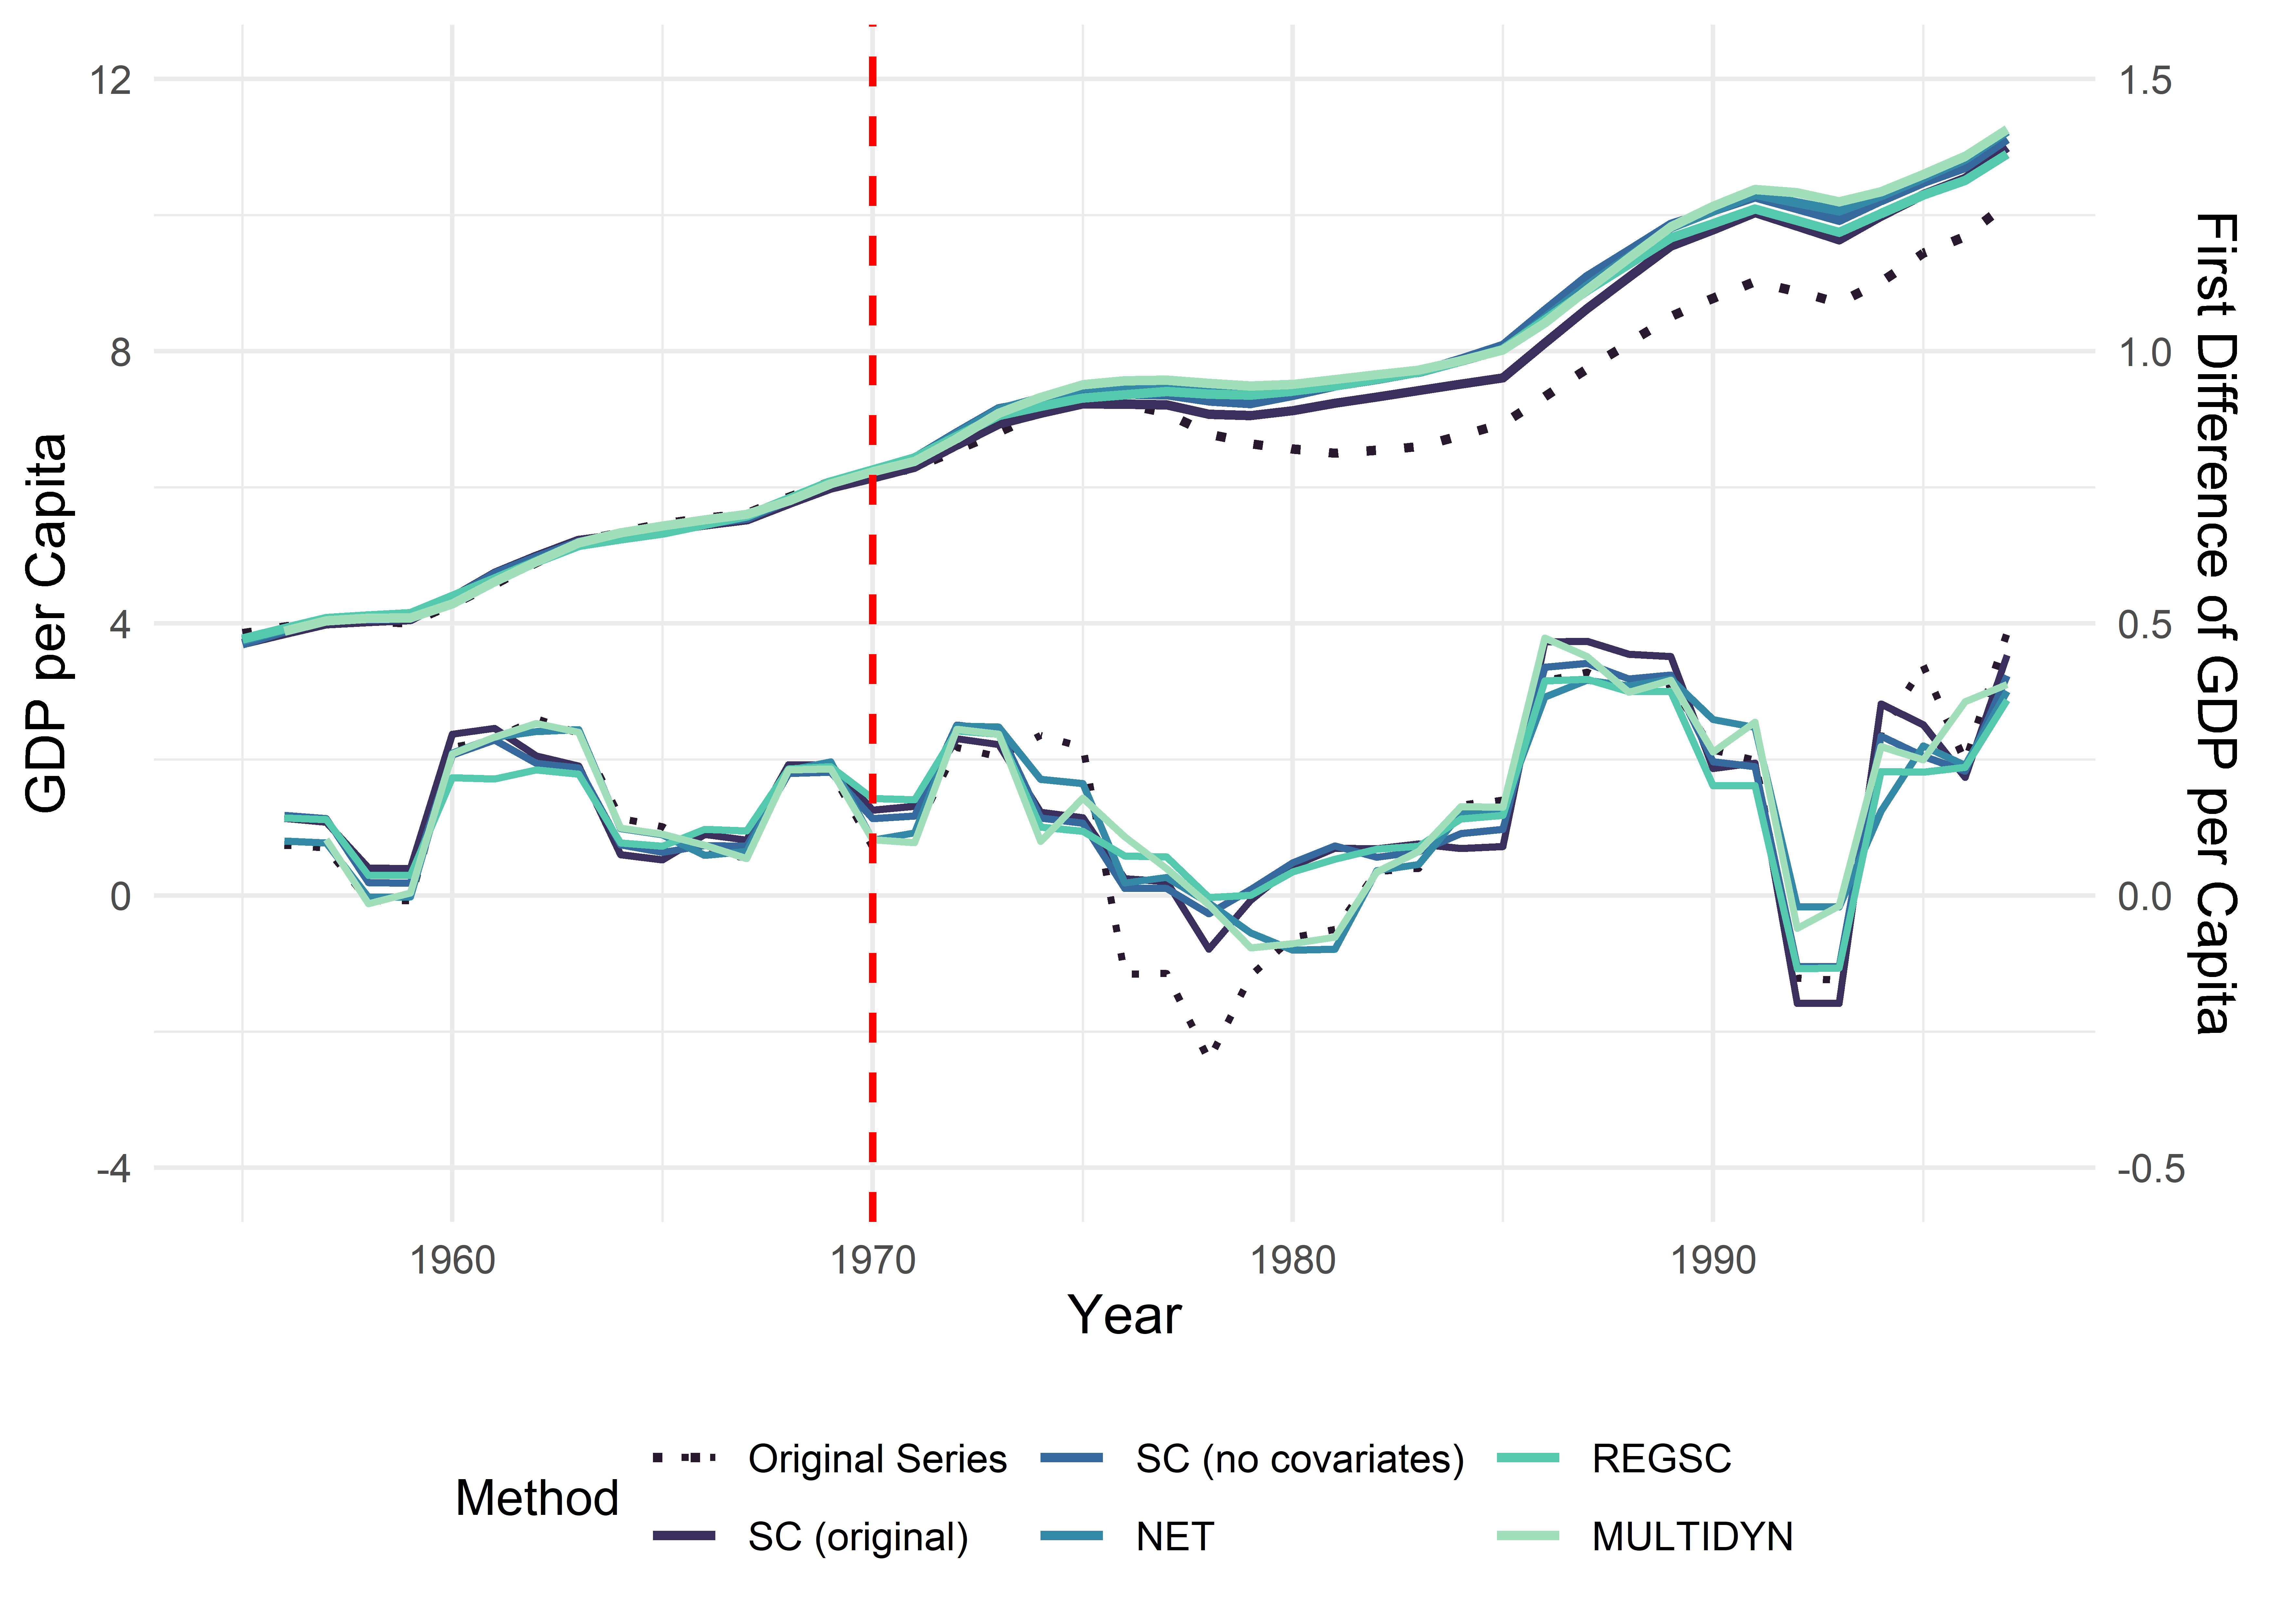
\includegraphics[scale=0.9]{F12}
	\caption{GDP per Capita for the (synthetic) Basque}
	\label{F_03}
\end{figure}

\newpage
\subsection{Estimating the Effect of California’s Tobacco Control Program}
\cite{abadie:2010}
\begin{figure}[H]
	\centering
	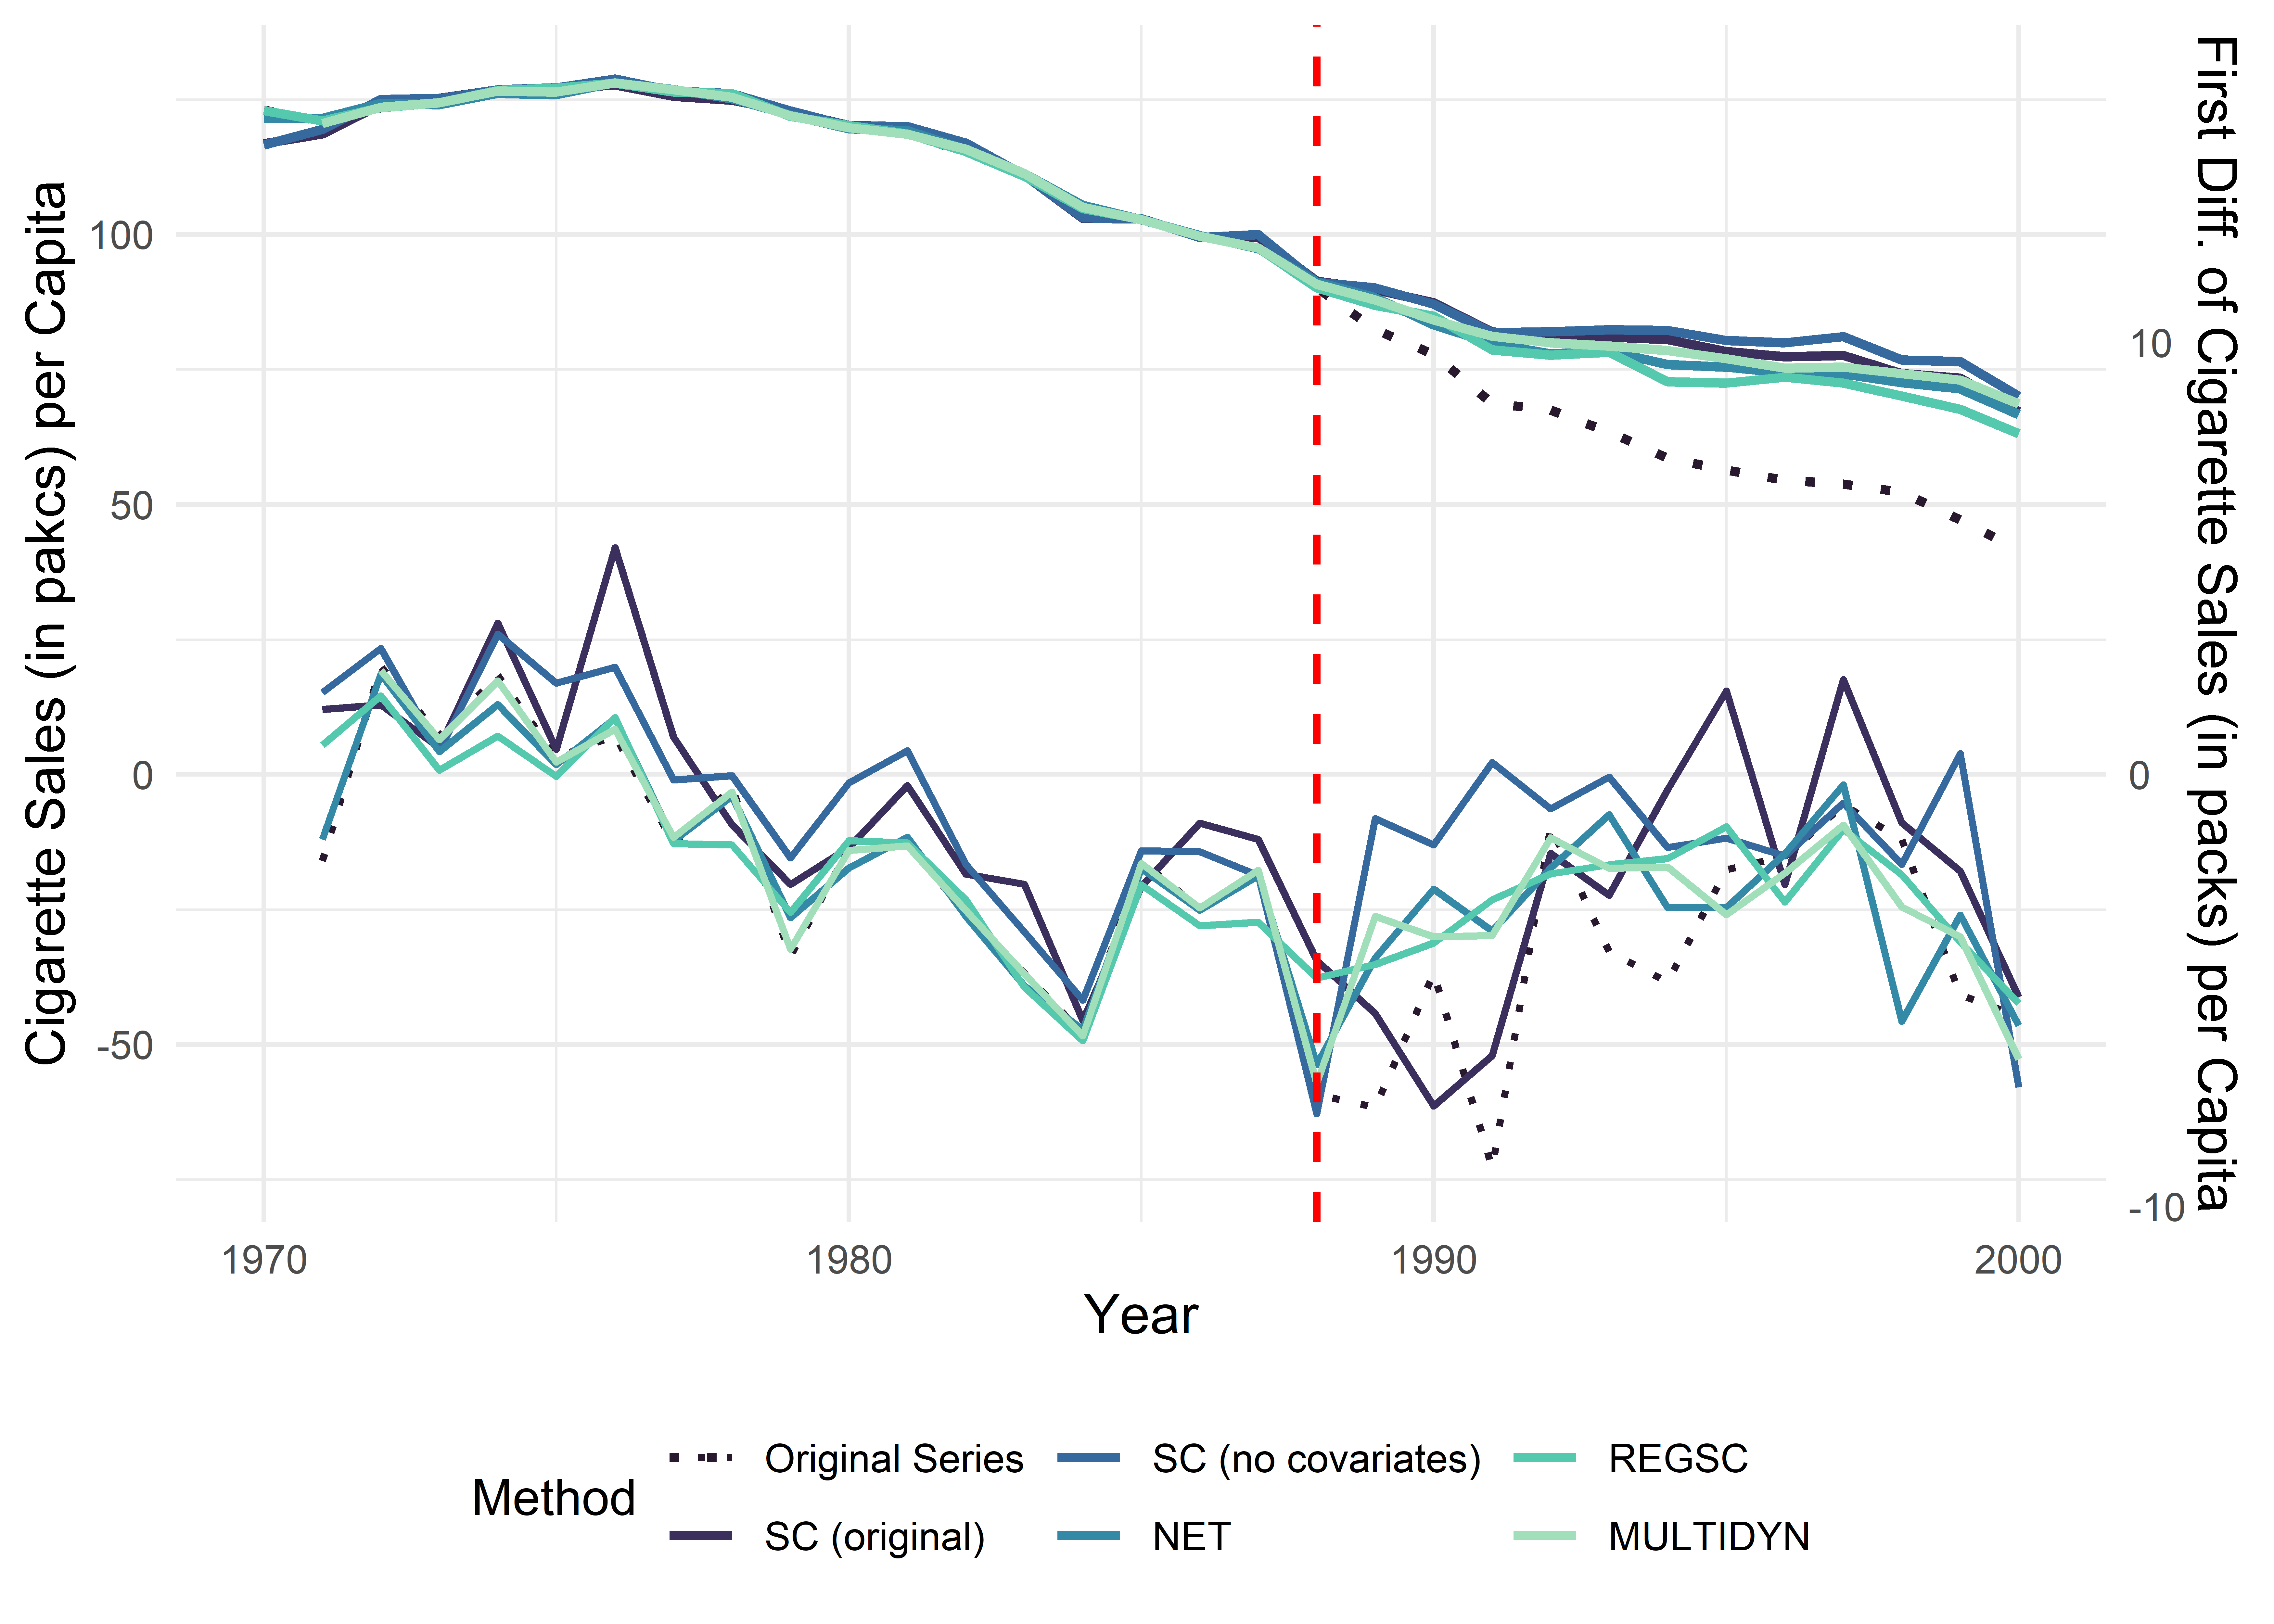
\includegraphics[scale=0.9]{F14}
	\caption{Cigarette Sales per Capita for the (synthetic) California}
	\label{F_04}
\end{figure}

\newpage
\subsection{The Economic Cost of the 1990 German Reunification}
\cite{abadie:2015}
\begin{figure}[H]
	\centering
	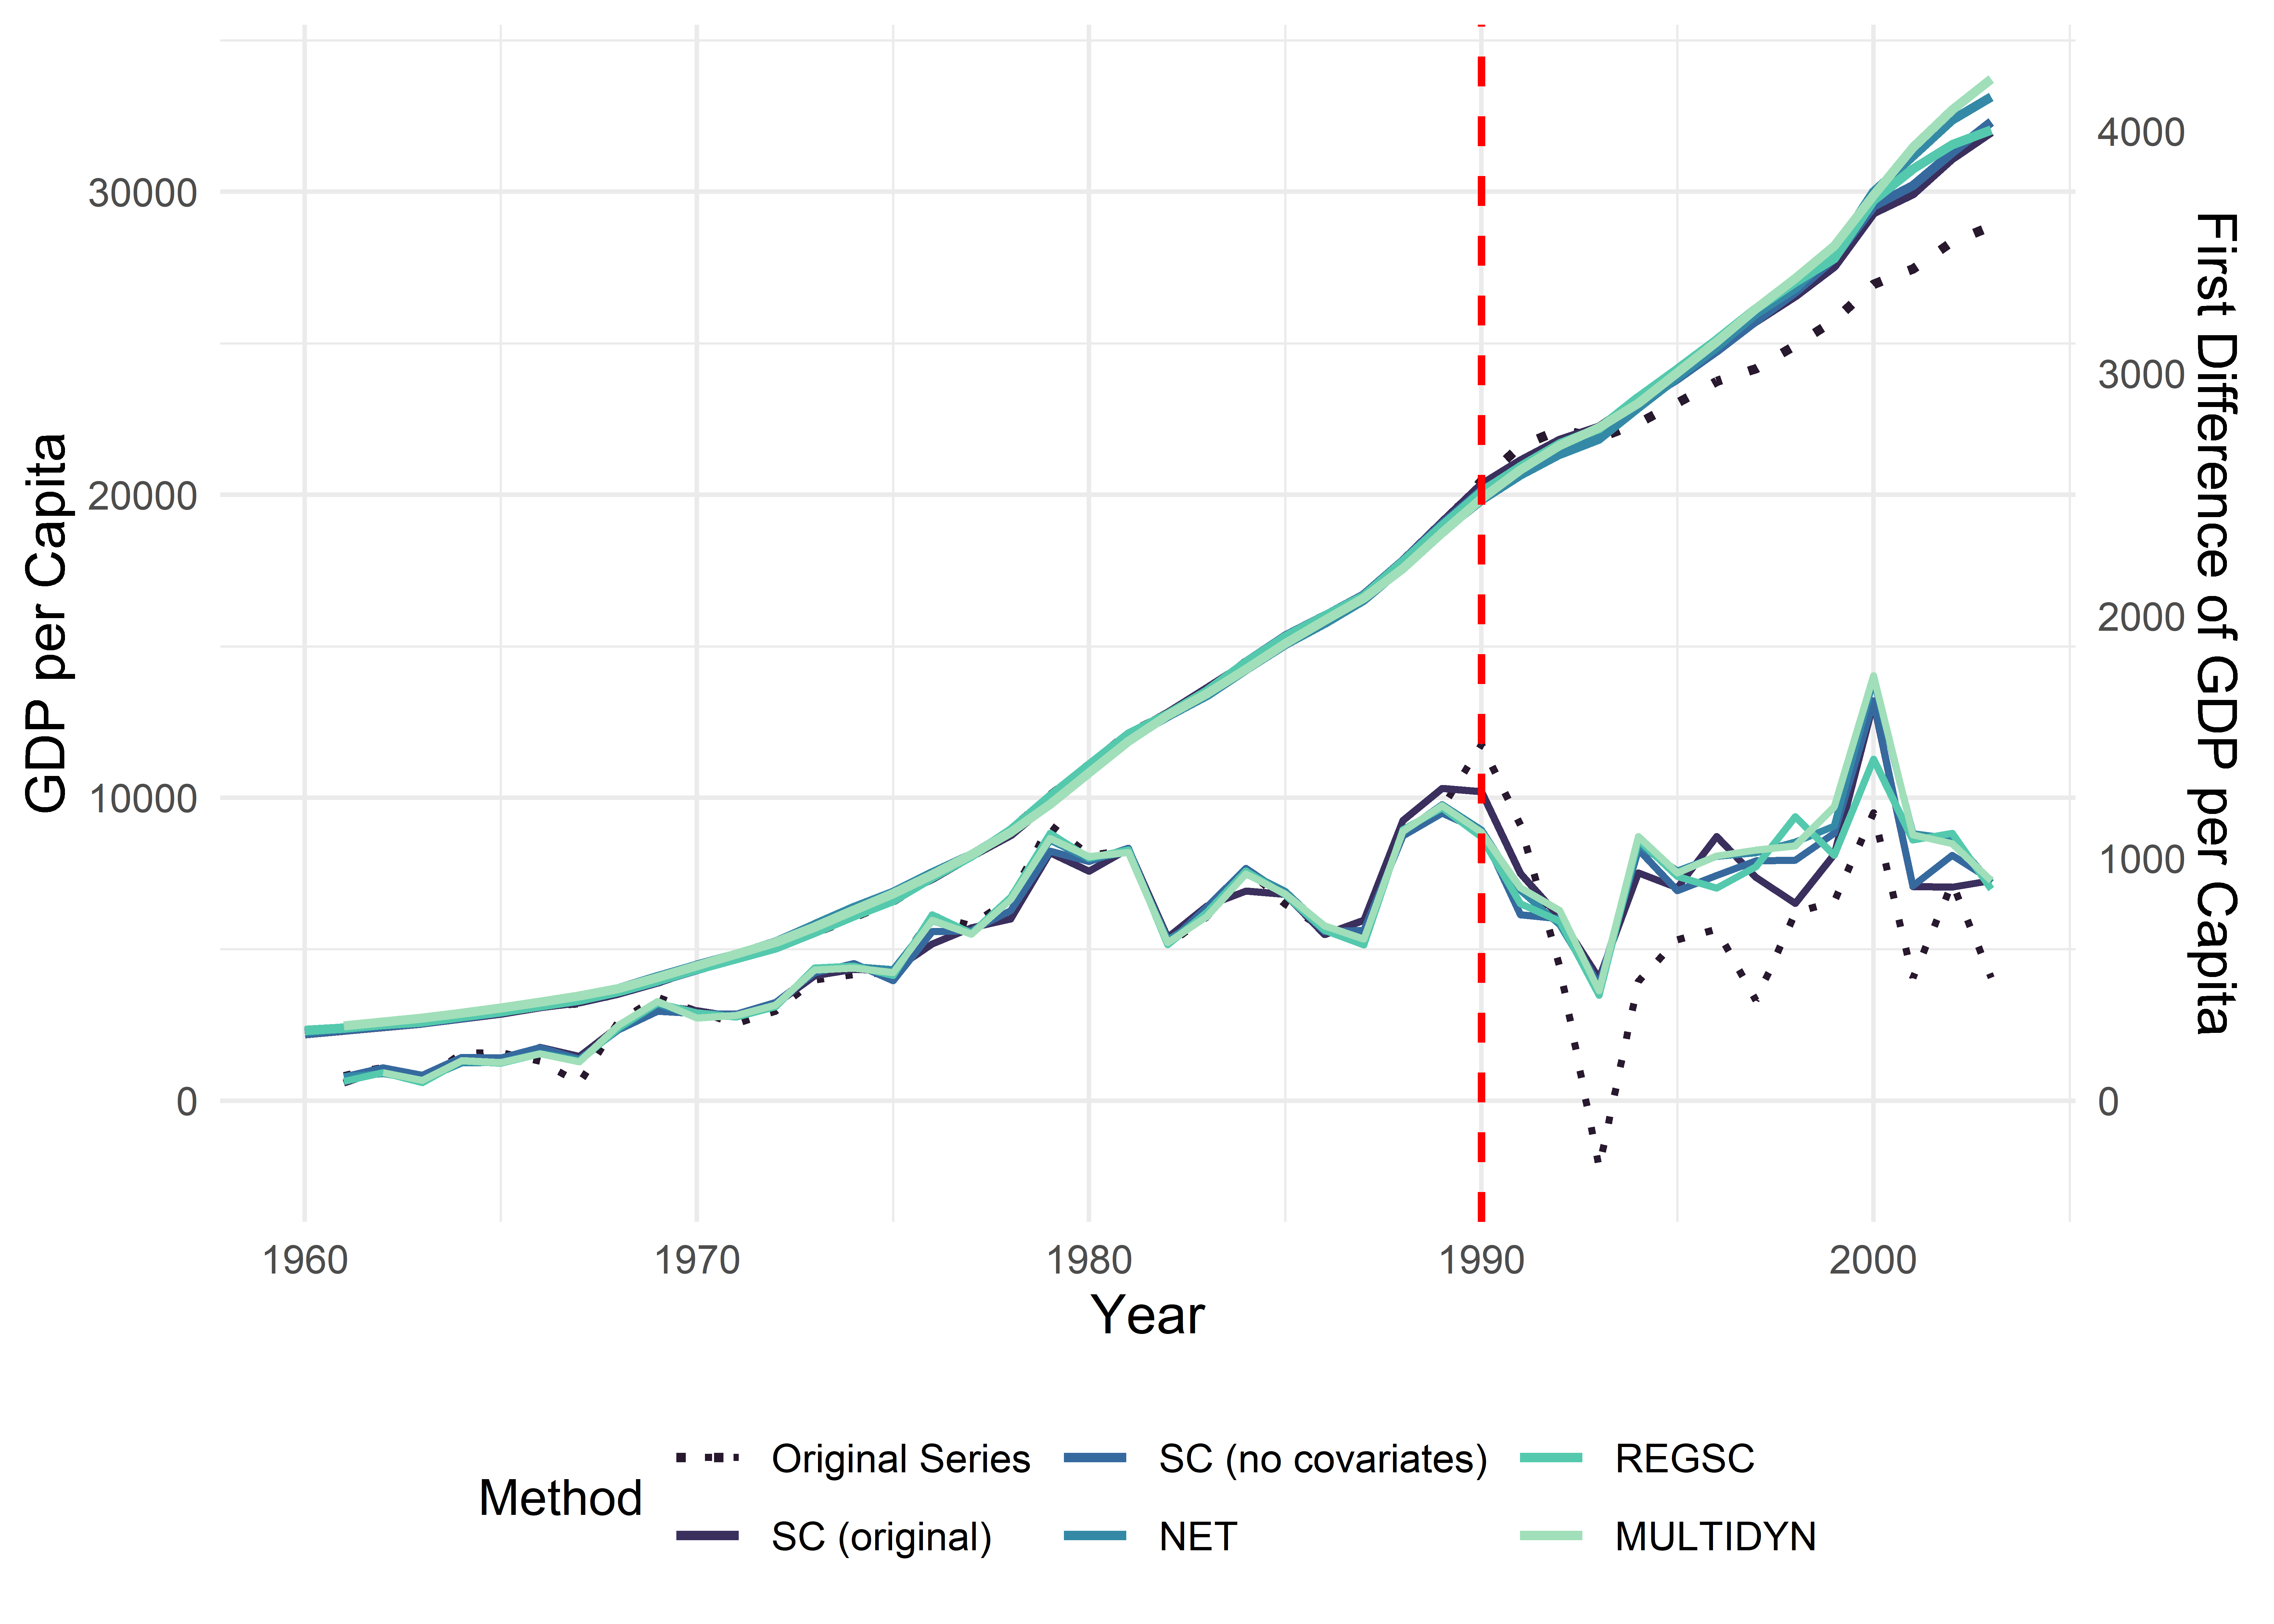
\includegraphics[scale=0.9]{F16}
	\caption{GDP per Capita for the (synthetic) West Germany}
	\label{F_05}
\end{figure}
	\newpage
	\section{Conclusion}
\begin{itemize}
	\item Some concluding remark and an outlook
	\item Keep short, around 1-2 pages
	\item Natural extension: case with explanatory variables
\end{itemize}
	
	\newpage
	\bibliographystyle{apalike} 
	\bibliography{mybib}
	
	\newpage
	\section{Appendix}
\subsection{Simple Static Extension}
\subsubsection{OLS Solution}
In case the population covariance matrix is observable, the OLS-coefficients can be directly derived from it: $\left( w_1^{OLS}, w_2^{OLS} \right) = \boldsymbol{\Sigma_2}^{-1} \boldsymbol{\sigma_{12}}  $
\subsubsection{SC Solution}
The restricted solution is can directly be derived from the covariance matrix. The first index in the square brackets indicates the row, the second the column position. 
\begin{equation*}
	\begin{split}
		w_1^{SC} & = \left( \boldsymbol{\sigma_{12}}^\prime[1] - \boldsymbol{\sigma_{12}}^\prime[2] - \boldsymbol{\Sigma_2}[2,1] + \boldsymbol{\Sigma_2}[1,1] \right) / \left( \boldsymbol{\Sigma_2}[1,1] + \boldsymbol{\Sigma_2}[2,2] - 2 * \boldsymbol{\Sigma_2}[1,2] \right) \\
		& = (0.1-0.4-0.5+1)/(1+1-2*0.5) = 0.2 
	\end{split} 
\end{equation*}
\begin{equation*}
	\begin{split}
		w_2^{SC} & = \left( \boldsymbol{\sigma_{12}}^\prime[2] - \boldsymbol{\sigma_{12}}^\prime[1] - \boldsymbol{\Sigma_2}[1,2] + \boldsymbol{\Sigma_2}[2,2] \right) / \left( \boldsymbol{\Sigma_2}[2,2] + \boldsymbol{\Sigma_2}[1,1] - 2 * \boldsymbol{\Sigma_2}[2,1] \right) \\
		& = (0.4-0.1-0.5+1)/(1+1-2*0.5) = 0.8
	\end{split}
\end{equation*}
\subsubsection{Variances}
The variances are derived from the weights and the covariance matrix:
\begin{equation*}
	\begin{split}
		var(Y_0 - w_1 Y_1 - w_2 Y_2) = &\text{ }var(Y_0) + w_1^2 \cdot var(Y_1) + w_2^2 \cdot var(Y_2)\text{ }- \\
		& 2 \cdot w_1 \cdot cov(Y_0, Y_1) - 2 \cdot w_2 \cdot cov(Y_0, Y_2)\text{ }+ \\
		&2 \cdot w_1 w_2 \cdot cov(Y_1, Y_2) 
	\end{split}
\end{equation*}

\newpage
\subsection{General Static Extension}
\subsubsection{REGSC: The limit for $\lambda_1\to \infty$ and $\lambda_2 \to \infty$}

For $\lambda_1\to \infty$ and $\lambda_2\to \infty$ the objective function reduce to
\begin{align*}
	Q(\lambda_1,\lambda2) &= \lambda_1 w'w + \lambda_2 (1-\mathbf{1}'w)^2
\end{align*}
The derivative is obtained as
\begin{align*}
	\frac{ \partial Q(\lambda_1,\lambda_2) }{ \partial w} &= 2 \lambda_1 w + 2 \lambda_2 (\mathbf{1}-\mathbf{1} \mathbf{1}'w)
\end{align*}
By setting the derivative to zero and multiplying with $\mathbf{1}$ we obtain:
\begin{align*}
	\lambda_1 \mathbf{1}'w + \lambda_2 (n- \mathbf{1}'w) = 0
\end{align*}
where $\mathbf{1}'w =\sum w_i$. Solving for $ \mathbf{1}'w $ we obtain
\begin{align*}
	\mathbf{1}'w  &= \frac{ 1}{ 1 +\lambda_1/\lambda_2 }
\end{align*}
and due to the symmetry of the objective function with respect to the elements of the weight vector we have
\begin{align*}
	w_i &= 1/(n+n\lambda_1/\lambda_2)
\end{align*}


\subsection{Simulation Study}
\subsubsection{Static Simulation results}
\label{Static simulation}
\newpage
\begin{table}[H]
	\centering
	\noindent
	\caption{Simulation Results of the Static Factor Model with \textbf{J = 5} Donors.}
	\scalebox{1}{
		\begin{tabular}{c c | C{2.48cm} | C{2.48cm} | C{2.48cm} | C{2.48cm} | C{2.48cm} }
			\toprule[1.5pt]
			\multicolumn{1}{c}{$\boldsymbol{T_{pre}}$} & \multicolumn{1}{c}{$\boldsymbol{T_{post}}$}& \multicolumn{1}{c}{\textbf{FACTOR}} & \multicolumn{1}{c}{\textbf{SC}} & \multicolumn{1}{c}{\textbf{REGSC}}& \multicolumn{1}{c}{\textbf{NET}}& \multicolumn{1}{c}{\textbf{OLS}}\\
			\cmidrule(lr){1-7}
			& & RMSE&RMSE&RMSE&RMSE&RMSE\\
			& & (BIAS)&(BIAS)&(BIAS)&(BIAS)&(BIAS)\\
			& & [MZ-RATES] & [MZ-RATES] & [MZ-RATES] &[MZ-RATES] &[MZ-RATES]\\
			& & \{VARIANCE\} & \{VARIANCE\}& \{VARIANCE\}&\{VARIANCE\} &\{VARIANCE\}\\
			\cmidrule(lr){1-7}
			20&30&1.2497&1.4455&1.3064&1.3086&1.3814\\
			&&(-0.0045)&(-0.0086)&(-0.0144)&(-0.0073)&(-0.0098)\\
			&&[0.7250]&[0.4210]&[0.6240]&[0.6691]&[0.5140]\\
			&&\{0.6523\}&\{1.1179\}&\{0.6898\}&\{0.6581\}&\{1.1678\}\\
			&20&1.2509&1.4575&1.3054&1.3048&1.3661\\
			&&(0.0137)&(0.0331)&(0.0063)&(0.0085)&(0.0114)\\
			&&[0.8240]&[0.5360]&[0.7460]&[0.7516]&[0.6650]\\
			&&\{0.6143\}&\{1.0690\}&\{0.6619\}&\{0.6137\}&\{1.1028\}\\
			&10&1.2344&1.4283&1.2847&1.2804&1.3520\\
			&&(-0.0092)&(-0.0120)&(-0.0075)&(-0.0098)&(-0.0126)\\
			&&[0.8940]&[0.7380]&[0.8540]&[0.8723]&[0.8060]\\
			&&\{0.6137\}&\{1.0366\}&\{0.6505\}&\{0.6086\}&\{1.0948\}\\
			\cmidrule(lr){1-7}
			% next specification
			50&30&1.1831&1.4185&1.2131&1.2045&1.2190\\
			&&(0.0147)&(-0.0223)&(0.0137)&(0.0117)&(0.0106)\\
			&&[0.8510]&[0.4600]&[0.8210]&[0.8388]&[0.8250]\\
			&&\{0.6459\}&\{1.0600\}&\{0.6440\}&\{0.5834\}&\{0.7974\}\\
			&20&1.1740&1.4160&1.2044&1.1948&1.2105\\
			&&(-0.0195)&(-0.0106)&(-0.0204)&(-0.0191)&(-0.0166)\\
			&&[0.9030]&[0.5630]&[0.8650]&[0.8810]&[0.8750]\\
			&&\{0.6426\}&\{1.0680\}&\{0.6311\}&\{0.5752\}&\{0.7879\}\\
			&10&1.1635&1.4033&1.1940&1.1845&1.2009\\
			&&(-0.0081)&(-0.0211)&(-0.0115)&(-0.0081)&(-0.0074)\\
			&&[0.9300]&[0.7340]&[0.9170]&[0.9260]&[0.9120]\\
			&&\{0.5963\}&\{1.0002\}&\{0.5850\}&\{0.5407\}&\{0.7415\}\\
			\cmidrule(lr){1-7}
			% next specification
			100&30&1.1645&1.3955&1.1811&1.1733&1.1799\\
			&&(0.0047)&(0.0381)&(0.0053)&(0.0048)&(0.0052)\\
			&&[0.8920]&[0.4950]&[0.8700]&[0.8930]&[0.8870]\\
			&&\{0.6494\}&\{1.0668\}&\{0.6405\}&\{0.5931\}&\{0.7238\}\\
			&20&1.1576&1.3796&1.1756&1.1691&1.1755\\
			&&(0.0026)&(-0.0384)&(0.0040)&(0.0021)&(0.0012)\\
			&&[0.9220]&[0.6080]&[0.9100]&[0.9120]&[0.9100]\\
			&&\{0.6389\}&\{1.0337\}&\{0.6226\}&\{0.5871\}&\{0.7090\}\\
			&10&1.1518&1.3907&1.1682&1.1643&1.1697\\
			&&(0.0108)&(0.0592)&(0.0156)&(0.0146)&(0.0135)\\
			&&[0.9440]&[0.7570]&[0.9370]&[0.9400]&[0.9330]\\
			&&\{0.5971\}&\{0.9826\}&\{0.5740\}&\{0.5432\}&\{0.6623\}\\
			\bottomrule[1.5pt]
	\end{tabular}}
	\label{table:table S.1}
\end{table}

\newpage
\begin{table}[H]
	\centering
	\noindent
	\caption{Simulation Results of the Static Factor Model with \textbf{J = 10} Donors.}
	\scalebox{1}{
		\begin{tabular}{c c | C{2.48cm} | C{2.48cm} | C{2.48cm} | C{2.48cm} | C{2.48cm} }
			\toprule[1.5pt]
			\multicolumn{1}{c}{$\boldsymbol{T_{pre}}$} & \multicolumn{1}{c}{$\boldsymbol{T_{post}}$}& \multicolumn{1}{c}{\textbf{FACTOR}} & \multicolumn{1}{c}{\textbf{SC}} & \multicolumn{1}{c}{\textbf{REGSC}}& \multicolumn{1}{c}{\textbf{NET}}& \multicolumn{1}{c}{\textbf{OLS}}\\
			\cmidrule(lr){1-7}
			& & RMSE&RMSE&RMSE&RMSE&RMSE\\
			& & (BIAS)&(BIAS)&(BIAS)&(BIAS)&(BIAS)\\
			& & [MZ-RATES] & [MZ-RATES] & [MZ-RATES] &[MZ-RATES] &[MZ-RATES]\\
			& & \{VARIANCE\} & \{VARIANCE\}& \{VARIANCE\}&\{VARIANCE\} &\{VARIANCE\}\\
			\cmidrule(lr){1-7}
			20&30&1.1575&1.2944&1.2229&1.2521&1.6286\\
			&&(-0.0071)&(0.0002)&(-0.0047)&(-0.0093)&(0.0018)\\
			&&[0.7090]&[0.5720]&[0.6590]&[0.6416]&[0.1790]\\
			&&\{0.7830\}&\{1.0468\}&\{0.7805\}&\{0.7714\}&\{2.3061\}\\
			&20&1.1611&1.2759&1.2336&1.2591&1.6075\\
			&&(0.0060)&(0.0197)&(0.0071)&(0.0036)&(0.0045)\\
			&&[0.8220]&[0.6920]&[0.7590]&[0.7495]&[0.3520]\\
			&&\{0.7459\}&\{1.0523\}&\{0.7777\}&\{0.7613\}&\{2.1785\}\\
			&10&1.1675&1.2963&1.2318&1.2659&1.6276\\
			&&(0.0040)&(0.0127)&(0.0004)&(0.0006)&(0.0181)\\
			&&[0.8840]&[0.8050]&[0.8550]&[0.8513]&[0.6020]\\
			&&\{0.6883\}&\{0.9859\}&\{0.7180\}&\{0.6984\}&\{2.0705\}\\
			\cmidrule(lr){1-7}
			% next specification
			50&30&1.1048&1.2511&1.1444&1.1524&1.2140\\
			&&(0.0049)&(0.0020)&(0.0079)&(0.0065)&(0.0087)\\
			&&[0.8640]&[0.6680]&[0.8240]&[0.8310]&[0.7420]\\
			&&\{0.7755\}&\{1.0148\}&\{0.7207\}&\{0.6795\}&\{1.1008\}\\
			&20&1.0985&1.2416&1.1327&1.1417&1.2022\\
			&&(0.0047)&(0.0037)&(0.0029)&(0.0042)&(0.0028)\\
			&&[0.8870]&[0.7270]&[0.8750]&[0.8750]&[0.8190]\\
			&&\{0.7744\}&\{0.9962\}&\{0.7333\}&\{0.6573\}&\{1.0658\}\\
			&10&1.0838&1.2171&1.1183&1.1270&1.1857\\
			&&(0.0001)&(0.0033)&(-0.0039)&(-0.0034)&(-0.0049)\\
			&&[0.9310]&[0.8560]&[0.9370]&[0.9290]&[0.9100]\\
			&&\{0.7704\}&\{0.9989\}&\{0.7199\}&\{0.6649\}&\{1.0604\}\\
			\cmidrule(lr){1-7}
			% next specification
			100&30&1.0920&1.2323&1.1141&1.1171&1.1405\\
			&&(0.0040)&(0.0119)&(0.0050)&(0.0039)&(0.0025)\\
			&&[0.9070]&[0.6930]&[0.9040]&[0.9080]&[0.8780]\\
			&&\{0.8025\}&\{1.0112\}&\{0.7620\}&\{0.6968\}&\{0.9363\}\\
			&20&1.0842&1.2232&1.1073&1.1088&1.1333\\
			&&(-0.0057)&(-0.0031)&(-0.0049)&(-0.0064)&(-0.0081)\\
			&&[0.9360]&[0.7680]&[0.9240]&[0.9280]&[0.9150]\\
			&&\{0.7858\}&\{1.0095\}&\{0.7427\}&\{0.6902\}&\{0.9314\}\\
			&10&1.0742&1.2059&1.0919&1.0986&1.1186\\
			&&(0.0080)&(-0.0206)&(0.0021)&(0.0016)&(0.0006)\\
			&&[0.9400]&[0.8660]&[0.9340]&[0.9470]&[0.9430]\\
			&&\{0.7377\}&\{0.9476\}&\{0.6925\}&\{0.6526\}&\{0.8653\}\\
			\bottomrule[1.5pt]
	\end{tabular}}
	\label{table:table S.2}
\end{table}

\newpage
\begin{table}[H]
	\centering
	\noindent
	\caption{Simulation Results of the Static Factor Model with \textbf{J = 15} Donors.}
	\scalebox{1}{
		\begin{tabular}{c c | C{2.48cm} | C{2.48cm} | C{2.48cm} | C{2.48cm} | C{2.48cm} }
			\toprule[1.5pt]
			\multicolumn{1}{c}{$\boldsymbol{T_{pre}}$} & \multicolumn{1}{c}{$\boldsymbol{T_{post}}$}& \multicolumn{1}{c}{\textbf{FACTOR}} & \multicolumn{1}{c}{\textbf{SC}} & \multicolumn{1}{c}{\textbf{REGSC}}& \multicolumn{1}{c}{\textbf{NET}}& \multicolumn{1}{c}{\textbf{OLS}}\\
			\cmidrule(lr){1-7}
			& & RMSE&RMSE&RMSE&RMSE&RMSE\\
			& & (BIAS)&(BIAS)&(BIAS)&(BIAS)&(BIAS)\\
			& & [MZ-RATES] & [MZ-RATES] & [MZ-RATES] &[MZ-RATES] &[MZ-RATES]\\
			& & \{VARIANCE\} & \{VARIANCE\}& \{VARIANCE\}&\{VARIANCE\} &\{VARIANCE\}\\
			\cmidrule(lr){1-7}
			20&30&1.1398&1.2604&1.2276&1.2533&2.4777\\
			&&(0.0243)&(0.0374)&(0.0244)&(0.0197)&(0.0312)\\
			&&[0.7340]&[0.6240]&[0.6450]&[0.6408]&[0.0320]\\
			&&\{0.7617\}&\{1.0341\}&\{0.8403\}&\{0.7997\}&\{6.3624\}\\
			&20&1.1287&1.2417&1.2149&1.2432&2.4716\\
			&&(0.0042)&(0.0258)&(0.0129)&(0.0165)&(-0.0097)\\
			&&[0.8200]&[0.7250]&[0.7460]&[0.7386]&[0.0690]\\
			&&\{0.7481\}&\{0.9966\}&\{0.8261\}&\{0.7667\}&\{6.3819\}\\
			&10&1.1112&1.2309&1.1973&1.2167&2.4393\\
			&&(0.0206)&(-0.0240)&(0.0224)&(0.0247)&(0.0245)\\
			&&[0.9030]&[0.8540]&[0.8640]&[0.8660]&[0.2450]\\
			&&\{0.7130\}&\{0.9484\}&\{0.7702\}&\{0.7234\}&\{6.0769\}\\
			\cmidrule(lr){1-7}
			% next specification
			50&30&1.0818&1.1935&1.1198&1.1356&1.2747\\
			&&(-0.0032)&(0.0006)&(-0.0019)&(-0.0019)&(-0.0040)\\
			&&[0.8580]&[0.7490]&[0.8230]&[0.8070]&[0.5980]\\
			&&\{0.8282\}&\{1.0035\}&\{0.7778\}&\{0.7102\}&\{1.3448\}\\
			&20&1.0879&1.1975&1.1307&1.1470&1.2892\\
			&&(-0.0133)&(-0.0183)&(-0.0205)&(-0.0188)&(-0.0210)\\
			&&[0.8950]&[0.8060]&[0.8710]&[0.8760]&[0.6930]\\
			&&\{0.7705\}&\{0.9465\}&\{0.7340\}&\{0.6722\}&\{1.2960\}\\
			&10&1.0522&1.1754&1.0896&1.1004&1.2281\\
			&&(-0.0132)&(-0.0098)&(-0.0130)&(-0.0122)&(-0.0011)\\
			&&[0.9240]&[0.8650]&[0.9170]&[0.9210]&[0.8460]\\
			&&\{0.7913\}&\{0.9519\}&\{0.7423\}&\{0.6776\}&\{1.2605\}\\
			\cmidrule(lr){1-7}
			% next specification
			100&30&1.0678&1.1818&1.0890&1.0974&1.1415\\
			&&(0.0007)&(-0.0212)&(0.0007)&(-0.0004)&(-0.0034)\\
			&&[0.8950]&[0.7310]&[0.8900]&[0.8730]&[0.8310]\\
			&&\{0.8395\}&\{0.9981\}&\{0.7767\}&\{0.7073\}&\{1.0481\}\\
			&20&1.0667&1.1809&1.0886&1.0947&1.1468\\
			&&(0.0048)&(-0.0018)&(0.0073)&(0.0064)&(0.0066)\\
			&&[0.9290]&[0.8040]&[0.9230]&[0.9180]&[0.8800]\\
			&&\{0.8321\}&\{0.9770\}&\{0.7671\}&\{0.6998\}&\{1.0384\}\\
			&10&1.0411&1.1459&1.0654&1.0717&1.1200\\
			&&(-0.0059)&(-0.0049)&(-0.0045)&(-0.0057)&(-0.0056)\\
			&&[0.9310]&[0.8740]&[0.9290]&[0.9290]&[0.9120]\\
			&&\{0.7897\}&\{0.9161\}&\{0.7422\}&\{0.6802\}&\{0.9948\}\\
			\bottomrule[1.5pt]
	\end{tabular}}
	\label{table:table S.3}
\end{table}

\newpage
\begin{table}[H]
	\centering
	\noindent
	\caption{Simulation Results of the Static Factor Model with \textbf{J = 20} Donors.}
	\scalebox{1}{
		\begin{tabular}{c c | C{2.48cm} | C{2.48cm} | C{2.48cm} | C{2.48cm} | C{2.48cm} }
			\toprule[1.5pt]
			\multicolumn{1}{c}{$\boldsymbol{T_{pre}}$} & \multicolumn{1}{c}{$\boldsymbol{T_{post}}$}& \multicolumn{1}{c}{\textbf{FACTOR}} & \multicolumn{1}{c}{\textbf{SC}} & \multicolumn{1}{c}{\textbf{REGSC}}& \multicolumn{1}{c}{\textbf{NET}}& \multicolumn{1}{c}{\textbf{OLS}}\\
			\cmidrule(lr){1-7}
			& & RMSE&RMSE&RMSE&RMSE&RMSE\\
			& & (BIAS)&(BIAS)&(BIAS)&(BIAS)&(BIAS)\\
			& & [MZ-RATES] & [MZ-RATES] & [MZ-RATES] &[MZ-RATES] &[MZ-RATES]\\
			& & \{VARIANCE\} & \{VARIANCE\}& \{VARIANCE\}&\{VARIANCE\} &\{VARIANCE\}\\
			\cmidrule(lr){1-7}
			20&30&1.1228&1.2229&1.2040&1.2331&NA\\
			&&(0.0074)&(-0.0229)&(0.0044)&(-0.0010)&(NA)\\
			&&[0.7090]&[0.6550]&[0.6410]&[0.6079]&[NA]\\
			&&\{0.8229\}&\{1.0024\}&\{0.8544\}&\{0.8238\}&\{NA\}\\
			&20&1.1230&1.2276&1.2093&1.2385&NA\\
			&&(0.0009)&(-0.0067)&(-0.0008)&(-0.0041)&(NA)\\
			&&[0.8030]&[0.7520]&[0.7250]&[0.7144]&[NA]\\
			&&\{0.7731\}&\{0.9833\}&\{0.8563\}&\{0.8207\}&\{NA\}\\
			&10&1.0939&1.1927&1.1749&1.2036&NA\\
			&&(0.0023)&(-0.0226)&(0.0033)&(0.0031)&(NA)\\
			&&[0.8860]&[0.8730]&[0.8480]&[0.8357]&[NA]\\
			&&\{0.7695\}&\{0.9365\}&\{0.8217\}&\{0.7697\}&\{NA\}\\
			\cmidrule(lr){1-7}
			% next specification
			50&30&1.0662&1.1629&1.1007&1.1180&1.3564\\
			&&(-0.0121)&(-0.0148)&(-0.0141)&(-0.0182)&(-0.0184)\\
			&&[0.8640]&[0.7290]&[0.8330]&[0.8230]&[0.4080]\\
			&&\{0.8580\}&\{0.9743\}&\{0.7912\}&\{0.7118\}&\{1.6096\}\\
			&20&1.0702&1.1693&1.1085&1.1205&1.3538\\
			&&(0.0004)&(0.0055)&(-0.0004)&(0.0008)&(-0.0073)\\
			&&[0.8810]&[0.8070]&[0.8710]&[0.8690]&[0.5880]\\
			&&\{0.8213\}&\{0.9484\}&\{0.7632\}&\{0.7049\}&\{1.5678\}\\
			&10&1.0566&1.1627&1.0907&1.1086&1.3371\\
			&&(0.0204)&(0.0143)&(0.0234)&(0.0242)&(0.0204)\\
			&&[0.9280]&[0.8950]&[0.9230]&[0.9230]&[0.8060]\\
			&&\{0.7780\}&\{0.9080\}&\{0.7208\}&\{0.6595\}&\{1.4765\}\\
			\cmidrule(lr){1-7}
			% next specification
			100&30&1.0512&1.1442&1.0735&1.0856&1.1639\\
			&&(-0.0083)&(0.0027)&(-0.0072)&(-0.0073)&(-0.0066)\\
			&&[0.9040]&[0.7800]&[0.8820]&[0.8890]&[0.7880]\\
			&&\{0.8556\}&\{0.9709\}&\{0.7933\}&\{0.7236\}&\{1.1355\}\\
			&20&1.0438&1.1434&1.0652&1.0763&1.1584\\
			&&(-0.0035)&(0.0063)&(-0.0009)&(-0.0030)&(-0.0035)\\
			&&[0.9230]&[0.8380]&[0.9260]&[0.9200]&[0.8400]\\
			&&\{0.8657\}&\{0.9643\}&\{0.7987\}&\{0.7379\}&\{1.1555\}\\
			&10&1.0381&1.1236&1.0615&1.0729&1.1502\\
			&&(-0.0014)&(-0.0054)&(0.0005)&(-0.0024)&(-0.0035)\\
			&&[0.9510]&[0.9110]&[0.9460]&[0.9380]&[0.9160]\\
			&&\{0.8044\}&\{0.8937\}&\{0.7387\}&\{0.6780\}&\{1.0692\}\\
			\bottomrule[1.5pt]
	\end{tabular}}
	\label{table:table S.4}
\end{table}

\newpage
\begin{table}[H]
	\centering
	\noindent
	\caption{Simulation Results of the Static Factor Model with \textbf{J = 25} Donors.}
	\scalebox{1}{
		\begin{tabular}{c c | C{2.48cm} | C{2.48cm} | C{2.48cm} | C{2.48cm} | C{2.48cm} }
			\toprule[1.5pt]
			\multicolumn{1}{c}{$\boldsymbol{T_{pre}}$} & \multicolumn{1}{c}{$\boldsymbol{T_{post}}$}& \multicolumn{1}{c}{\textbf{FACTOR}} & \multicolumn{1}{c}{\textbf{SC}} & \multicolumn{1}{c}{\textbf{REGSC}}& \multicolumn{1}{c}{\textbf{NET}}& \multicolumn{1}{c}{\textbf{OLS}}\\
			\cmidrule(lr){1-7}
			& & RMSE&RMSE&RMSE&RMSE&RMSE\\
			& & (BIAS)&(BIAS)&(BIAS)&(BIAS)&(BIAS)\\
			& & [MZ-RATES] & [MZ-RATES] & [MZ-RATES] &[MZ-RATES] &[MZ-RATES]\\
			& & \{VARIANCE\} & \{VARIANCE\}& \{VARIANCE\}&\{VARIANCE\} &\{VARIANCE\}\\
			\cmidrule(lr){1-7}
			20&30&1.1154&NA&1.2097&1.2225&NA\\
			&&(0.0019)&(NA)&(-0.0002)&(-0.0036)&(NA)\\
			&&[0.6980]&[NA]&[0.6280]&[0.6440]&[NA]\\
			&&\{0.8012\}&\{NA\}&\{0.8593\}&\{0.7918\}&\{NA\}\\
			&20&1.1038&NA&1.2001&1.2240&NA\\
			&&(0.0081)&(NA)&(0.0127)&(0.0125)&(NA)\\
			&&[0.8150]&[NA]&[0.7410]&[0.7310]&[NA]\\
			&&\{0.7882\}&\{NA\}&\{0.8314\}&\{0.7967\}&\{NA\}\\
			&10&1.1051&NA&1.1829&1.2061&NA\\
			&&(0.0056)&(NA)&(-0.0046)&(-0.0038)&(NA)\\
			&&[0.8830]&[NA]&[0.8590]&[0.8513]&[NA]\\
			&&\{0.7503\}&\{NA\}&\{0.7897\}&\{0.7621\}&\{NA\}\\
			\cmidrule(lr){1-7}
			% next specification
			50&30&1.0657&1.1525&1.1039&1.1198&1.4937\\
			&&(0.0104)&(-0.0014)&(0.0121)&(0.0119)&(0.0138)\\
			&&[0.8510]&[0.7880]&[0.8390]&[0.8270]&[0.2260]\\
			&&\{0.8576\}&\{0.9696\}&\{0.8090\}&\{0.7223\}&\{2.0239\}\\
			&20&1.0541&1.1514&1.0905&1.1090&1.4816\\
			&&(0.0175)&(0.0171)&(0.0202)&(0.0204)&(0.0229)\\
			&&[0.9000]&[0.8460]&[0.8840]&[0.8720]&[0.3860]\\
			&&\{0.8634\}&\{0.9776\}&\{0.8007\}&\{0.7497\}&\{2.0191\}\\
			&10&1.0513&1.1507&1.0911&1.1025&1.4816\\
			&&(-0.0003)&(0.0100)&(-0.0041)&(-0.0056)&(-0.0103)\\
			&&[0.9250]&[0.8930]&[0.9180]&[0.9260]&[0.6880]\\
			&&\{0.8091\}&\{0.9253\}&\{0.7763\}&\{0.7072\}&\{1.9764\}\\
			\cmidrule(lr){1-7}
			% next specification
			100&30&1.0377&1.1262&1.0607&1.0719&1.1913\\
			&&(-0.0036)&(0.0009)&(-0.0028)&(-0.0026)&(0.0002)\\
			&&[0.9190]&[0.8120]&[0.9070]&[0.9000]&[0.7200]\\
			&&\{0.8703\}&\{0.9562\}&\{0.7995\}&\{0.7252\}&\{1.2385\}\\
			&20&1.0431&1.1258&1.0656&1.0778&1.1897\\
			&&(-0.0088)&(-0.0108)&(-0.0075)&(-0.0084)&(-0.0028)\\
			&&[0.9220]&[0.8450]&[0.9180]&[0.9110]&[0.8160]\\
			&&\{0.8747\}&\{0.9594\}&\{0.8108\}&\{0.7317\}&\{1.2371\}\\
			&10&1.0240&1.1119&1.0478&1.0588&1.1803\\
			&&(-0.0011)&(0.0133)&(0.0015)&(0.0023)&(0.0046)\\
			&&[0.9330]&[0.9050]&[0.9250]&[0.9240]&[0.8930]\\
			&&\{0.8335\}&\{0.9086\}&\{0.7689\}&\{0.6957\}&\{1.1779\}\\
			\bottomrule[1.5pt]
	\end{tabular}}
	\label{table:table S.5}
\end{table}

\newpage
\begin{table}[H]
	\centering
	\noindent
	\caption{Simulation Results of the Static Factor Model with \textbf{J = 30} Donors.}
	\scalebox{1}{
		\begin{tabular}{c c | C{2.48cm} | C{2.48cm} | C{2.48cm} | C{2.48cm} | C{2.48cm} }
			\toprule[1.5pt]
			\multicolumn{1}{c}{$\boldsymbol{T_{pre}}$} & \multicolumn{1}{c}{$\boldsymbol{T_{post}}$}& \multicolumn{1}{c}{\textbf{FACTOR}} & \multicolumn{1}{c}{\textbf{SC}} & \multicolumn{1}{c}{\textbf{REGSC}}& \multicolumn{1}{c}{\textbf{NET}}& \multicolumn{1}{c}{\textbf{OLS}}\\
			\cmidrule(lr){1-7}
			& & RMSE&RMSE&RMSE&RMSE&RMSE\\
			& & (BIAS)&(BIAS)&(BIAS)&(BIAS)&(BIAS)\\
			& & [MZ-RATES] & [MZ-RATES] & [MZ-RATES] &[MZ-RATES] &[MZ-RATES]\\
			& & \{VARIANCE\} & \{VARIANCE\}& \{VARIANCE\}&\{VARIANCE\} &\{VARIANCE\}\\
			\cmidrule(lr){1-7}
			20&30&1.0985&NA&1.1867&1.2139&NA\\
			&&(0.0061)&(NA)&(0.0131)&(0.0104)&(NA)\\
			&&[0.7480]&[NA]&[0.6260]&[0.6397]&[NA]\\
			&&\{0.8283\}&\{NA\}&\{0.8679\}&\{0.8722\}&\{NA\}\\
			&20&1.0915&NA&1.1714&1.2129&NA\\
			&&(0.0044)&(NA)&(-0.0013)&(0.0022)&(NA)\\
			&&[0.8140]&[NA]&[0.7480]&[0.7409]&[NA]\\
			&&\{0.8092\}&\{NA\}&\{0.8365\}&\{0.8370\}&\{NA\}\\
			&10&1.0803&NA&1.1591&1.1885&NA\\
			&&(0.0225)&(NA)&(0.0147)&(0.0210)&(NA)\\
			&&[0.9060]&[NA]&[0.8560]&[0.8616]&[NA]\\
			&&\{0.7730\}&\{NA\}&\{0.8143\}&\{0.7921\}&\{NA\}\\
			\cmidrule(lr){1-7}
			% next specification
			50&30&1.0552&1.1492&1.0989&1.1206&1.6600\\
			&&(0.0048)&(0.0185)&(0.0050)&(0.0012)&(0.0062)\\
			&&[0.8600]&[0.8060]&[0.8220]&[0.8270]&[0.0960]\\
			&&\{0.8536\}&\{0.9671\}&\{0.7988\}&\{0.7556\}&\{2.5759\}\\
			&20&1.0488&1.1312&1.0819&1.1032&1.6398\\
			&&(0.0021)&(0.0090)&(-0.0005)&(-0.0001)&(-0.0045)\\
			&&[0.8990]&[0.8560]&[0.8680]&[0.8630]&[0.2330]\\
			&&\{0.8787\}&\{0.9519\}&\{0.8199\}&\{0.7509\}&\{2.5723\}\\
			&10&1.0381&1.1327&1.0792&1.0985&1.6269\\
			&&(0.0031)&(-0.0015)&(-0.0019)&(-0.0064)&(-0.0201)\\
			&&[0.9180]&[0.8910]&[0.9140]&[0.9100]&[0.5780]\\
			&&\{0.8092\}&\{0.8922\}&\{0.7594\}&\{0.6948\}&\{2.3713\}\\
			\cmidrule(lr){1-7}
			% next specification
			100&30&1.0460&1.1253&1.0709&1.0840&1.2419\\
			&&(0.0116)&(0.0154)&(0.0107)&(0.0118)&(0.0059)\\
			&&[0.9060]&[0.8500]&[0.9020]&[0.8890]&[0.6290]\\
			&&\{0.8951\}&\{0.9630\}&\{0.8098\}&\{0.7518\}&\{1.3709\}\\
			&20&1.0278&1.1067&1.0477&1.0626&1.2180\\
			&&(-0.0039)&(-0.0003)&(-0.0035)&(-0.0021)&(0.0002)\\
			&&[0.9380]&[0.8750]&[0.9270]&[0.9210]&[0.7660]\\
			&&\{0.9037\}&\{0.9668\}&\{0.8308\}&\{0.7497\}&\{1.3736\}\\
			&10&1.0300&1.0995&1.0509&1.0646&1.2299\\
			&&(-0.0309)&(-0.0335)&(-0.0339)&(-0.0330)&(-0.0419)\\
			&&[0.9330]&[0.9130]&[0.9240]&[0.9280]&[0.8660]\\
			&&\{0.8168\}&\{0.8818\}&\{0.7504\}&\{0.6825\}&\{1.2708\}\\
			\bottomrule[1.5pt]
	\end{tabular}}
	\label{table:table S.6}
\end{table}

\begin{figure}[H]
	\centering
	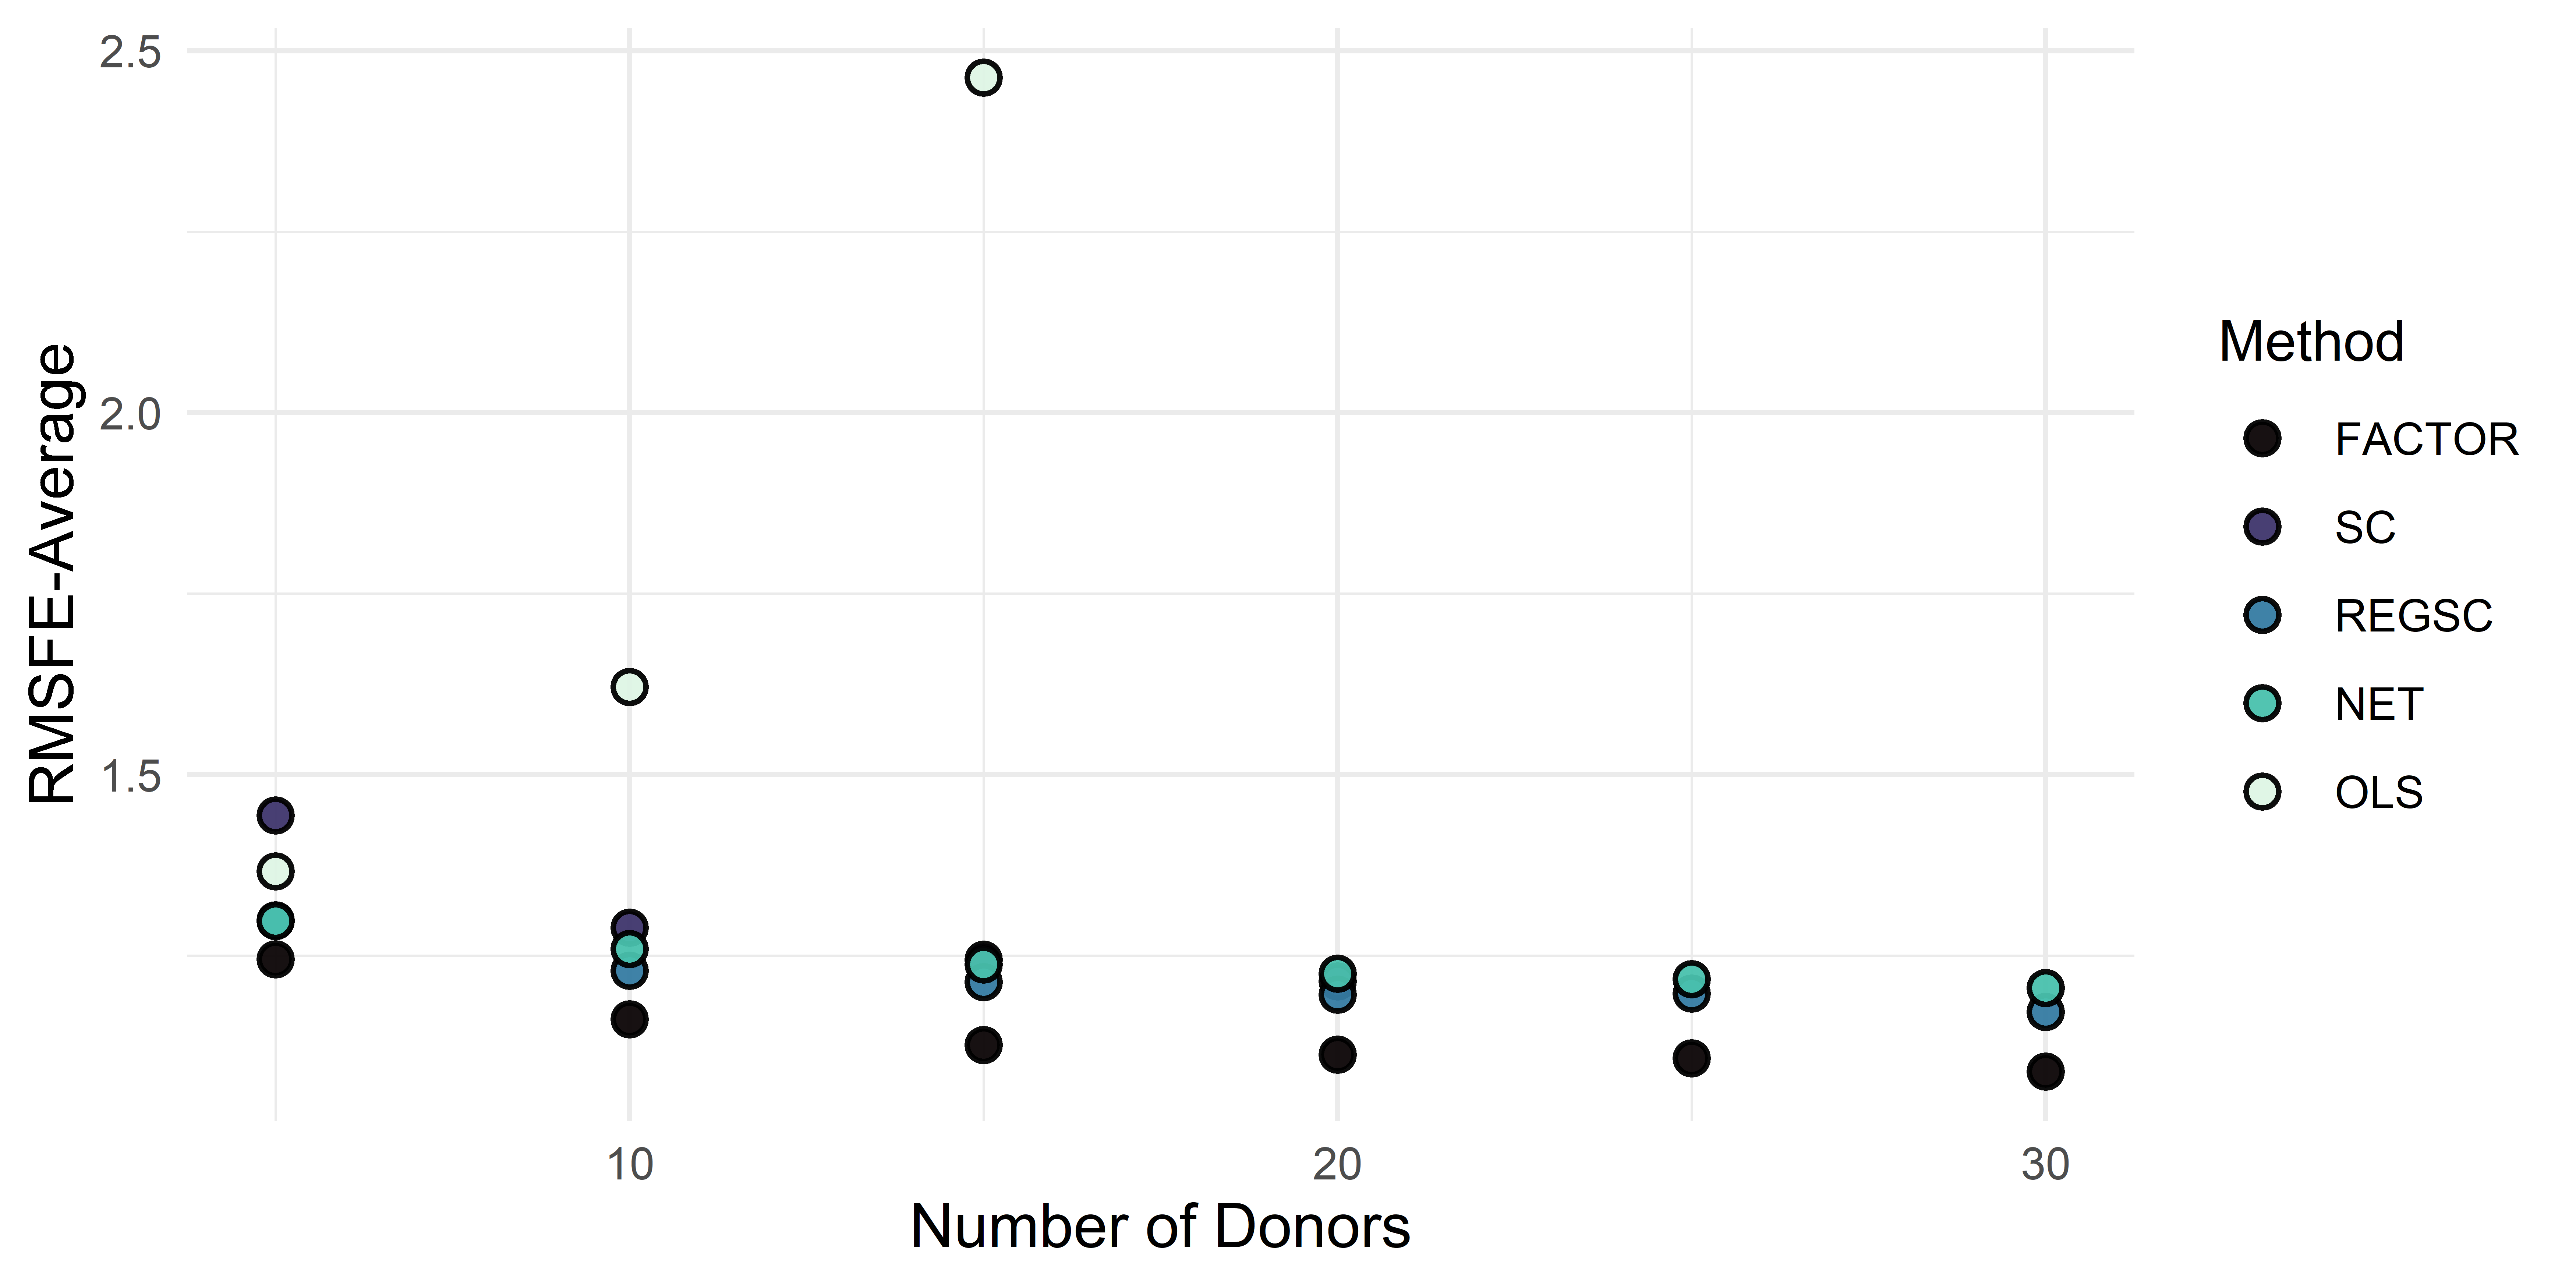
\includegraphics[scale=.9]{F06}
	\caption{Simulation Performance for $T_{pre} = 20$ and $T_{post} \in \left\lbrace 10,20,30\right\rbrace$}
	\label{F_10}
\end{figure}

\begin{figure}[H]
	\centering
	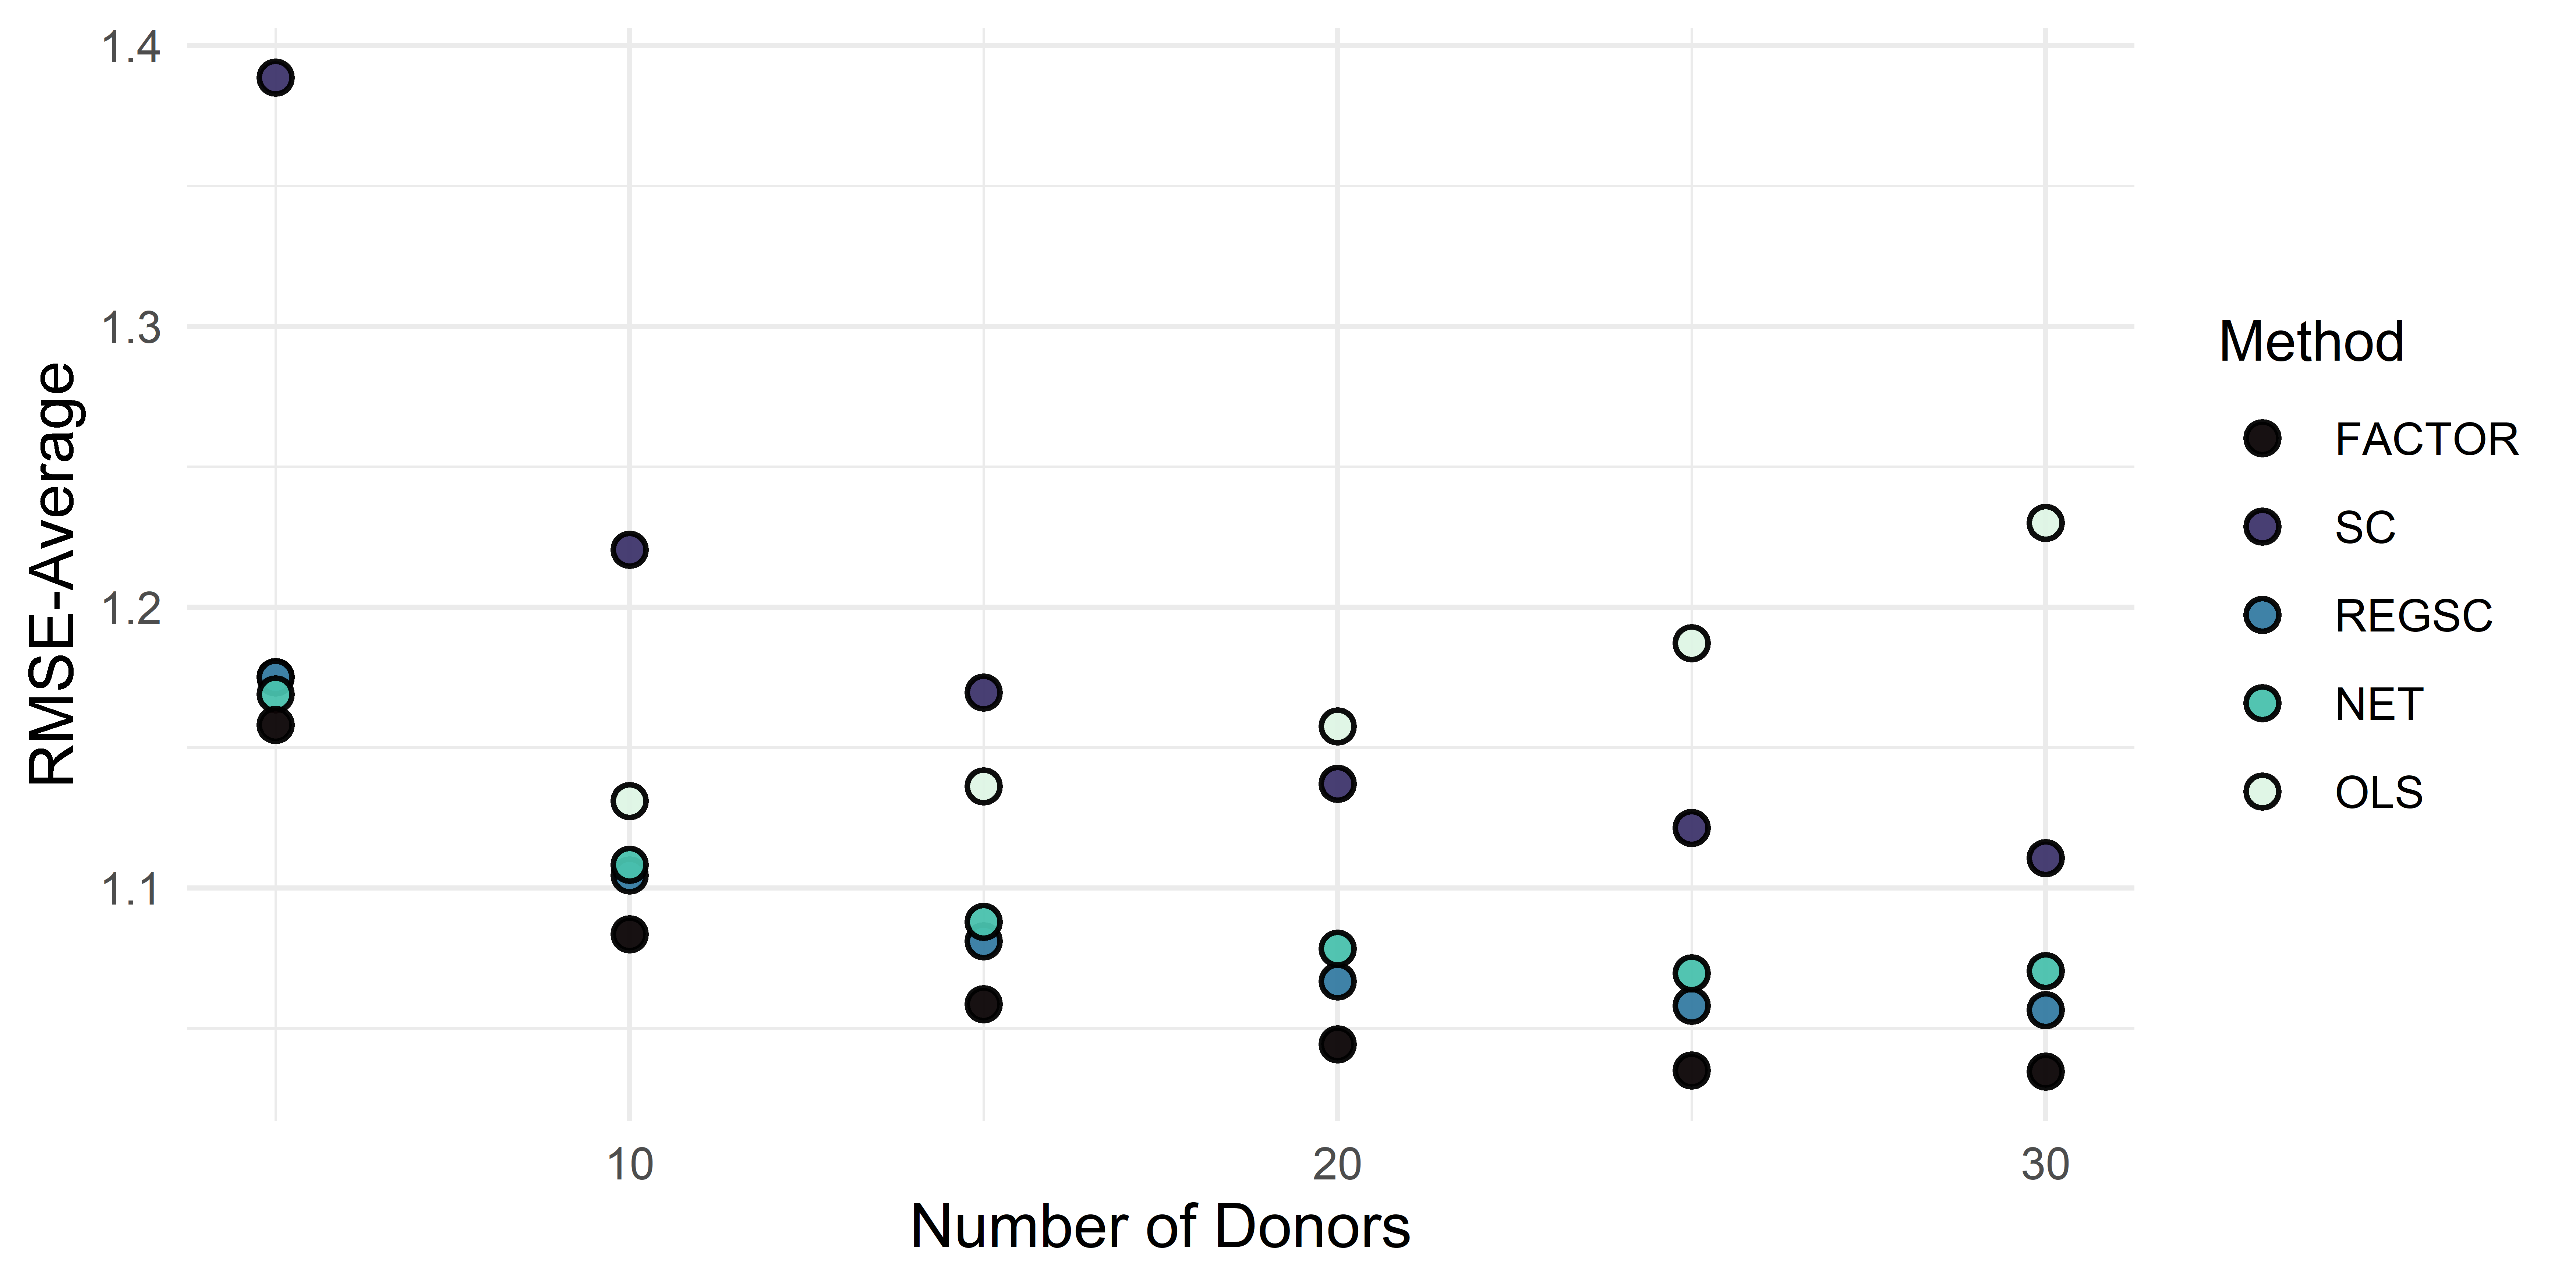
\includegraphics[scale=.9]{F08}
	\caption{Simulation Performance for $T_{pre} = 100$ and $T_{post} \in \left\lbrace 10,20,30\right\rbrace$}
	\label{F_11}
\end{figure}

\newpage
\begin{figure}[H]
	\centering
	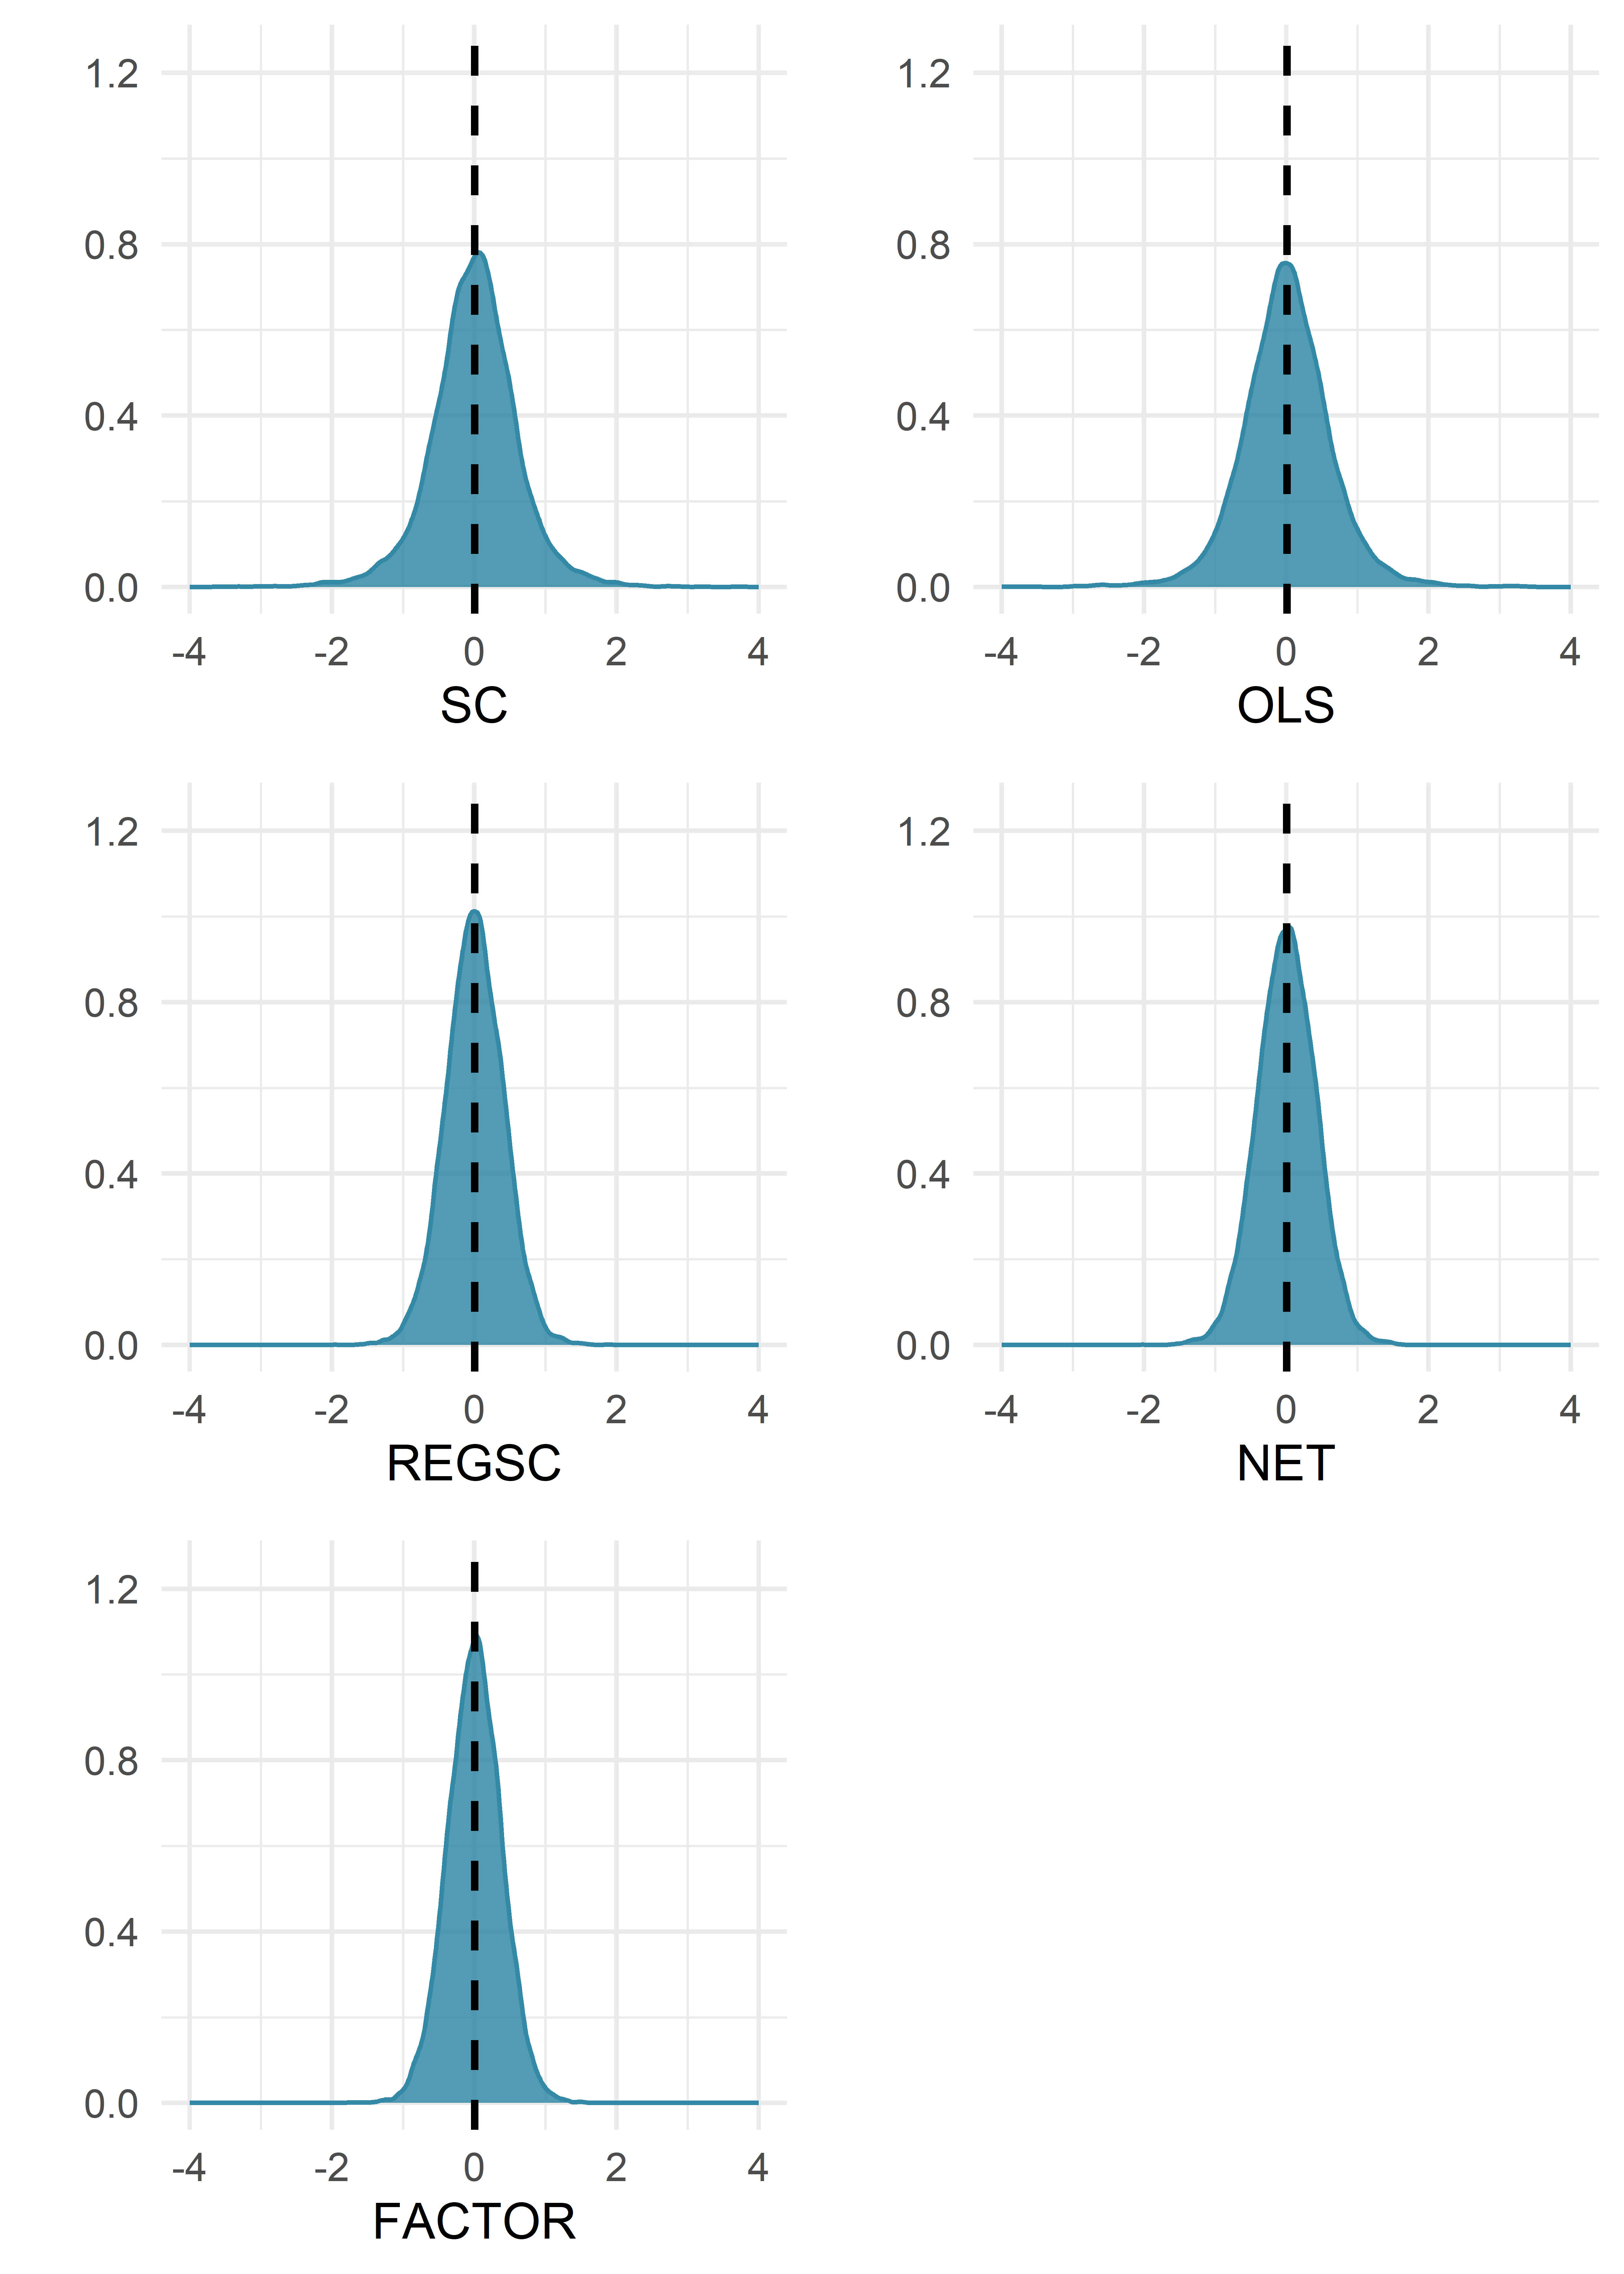
\includegraphics[scale=.9]{F17}
	\caption{Bias-densities for $T_{pre} = 20$ and $T_{post} \in \left\lbrace 10,20,30\right\rbrace$}
	\label{F_12}
\end{figure}

\newpage
\begin{figure}[H]
	\centering
	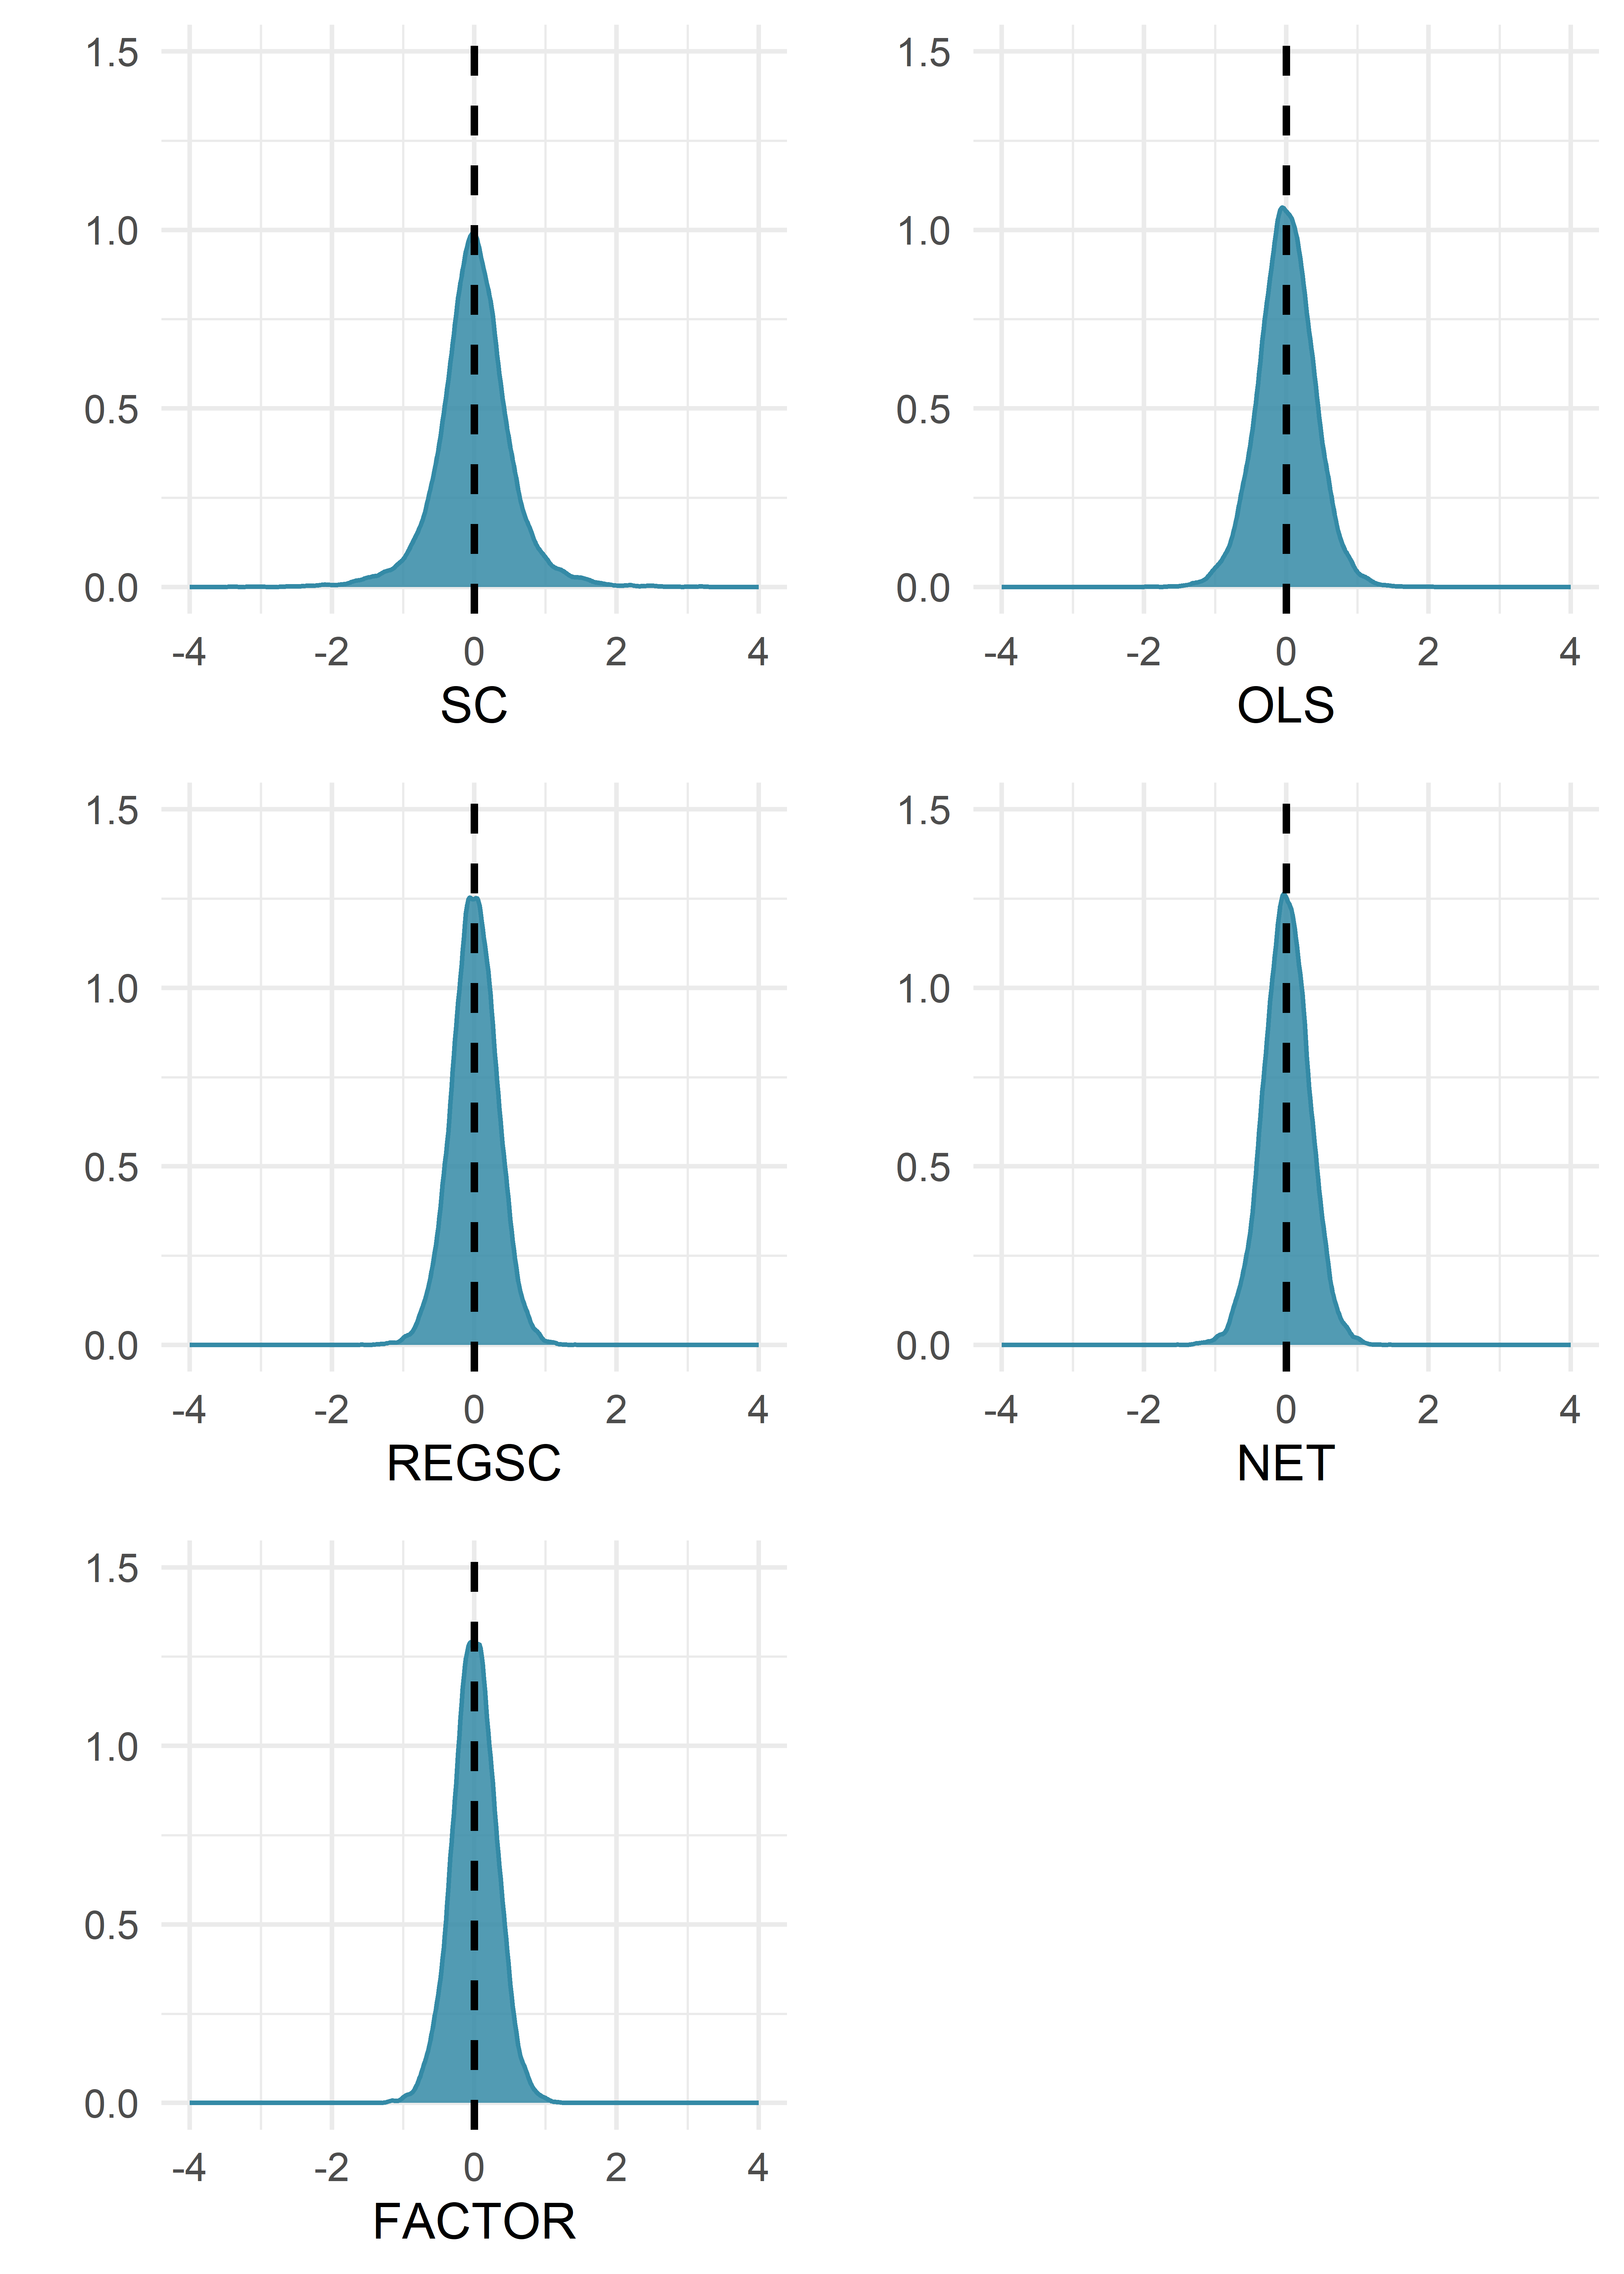
\includegraphics[scale=.9]{F18}
	\caption{Bias-densities for $T_{pre} = 50$ and $T_{post} \in \left\lbrace 10,20,30\right\rbrace$}
	\label{F_13}
\end{figure}

\newpage
\begin{figure}[H]
	\centering
	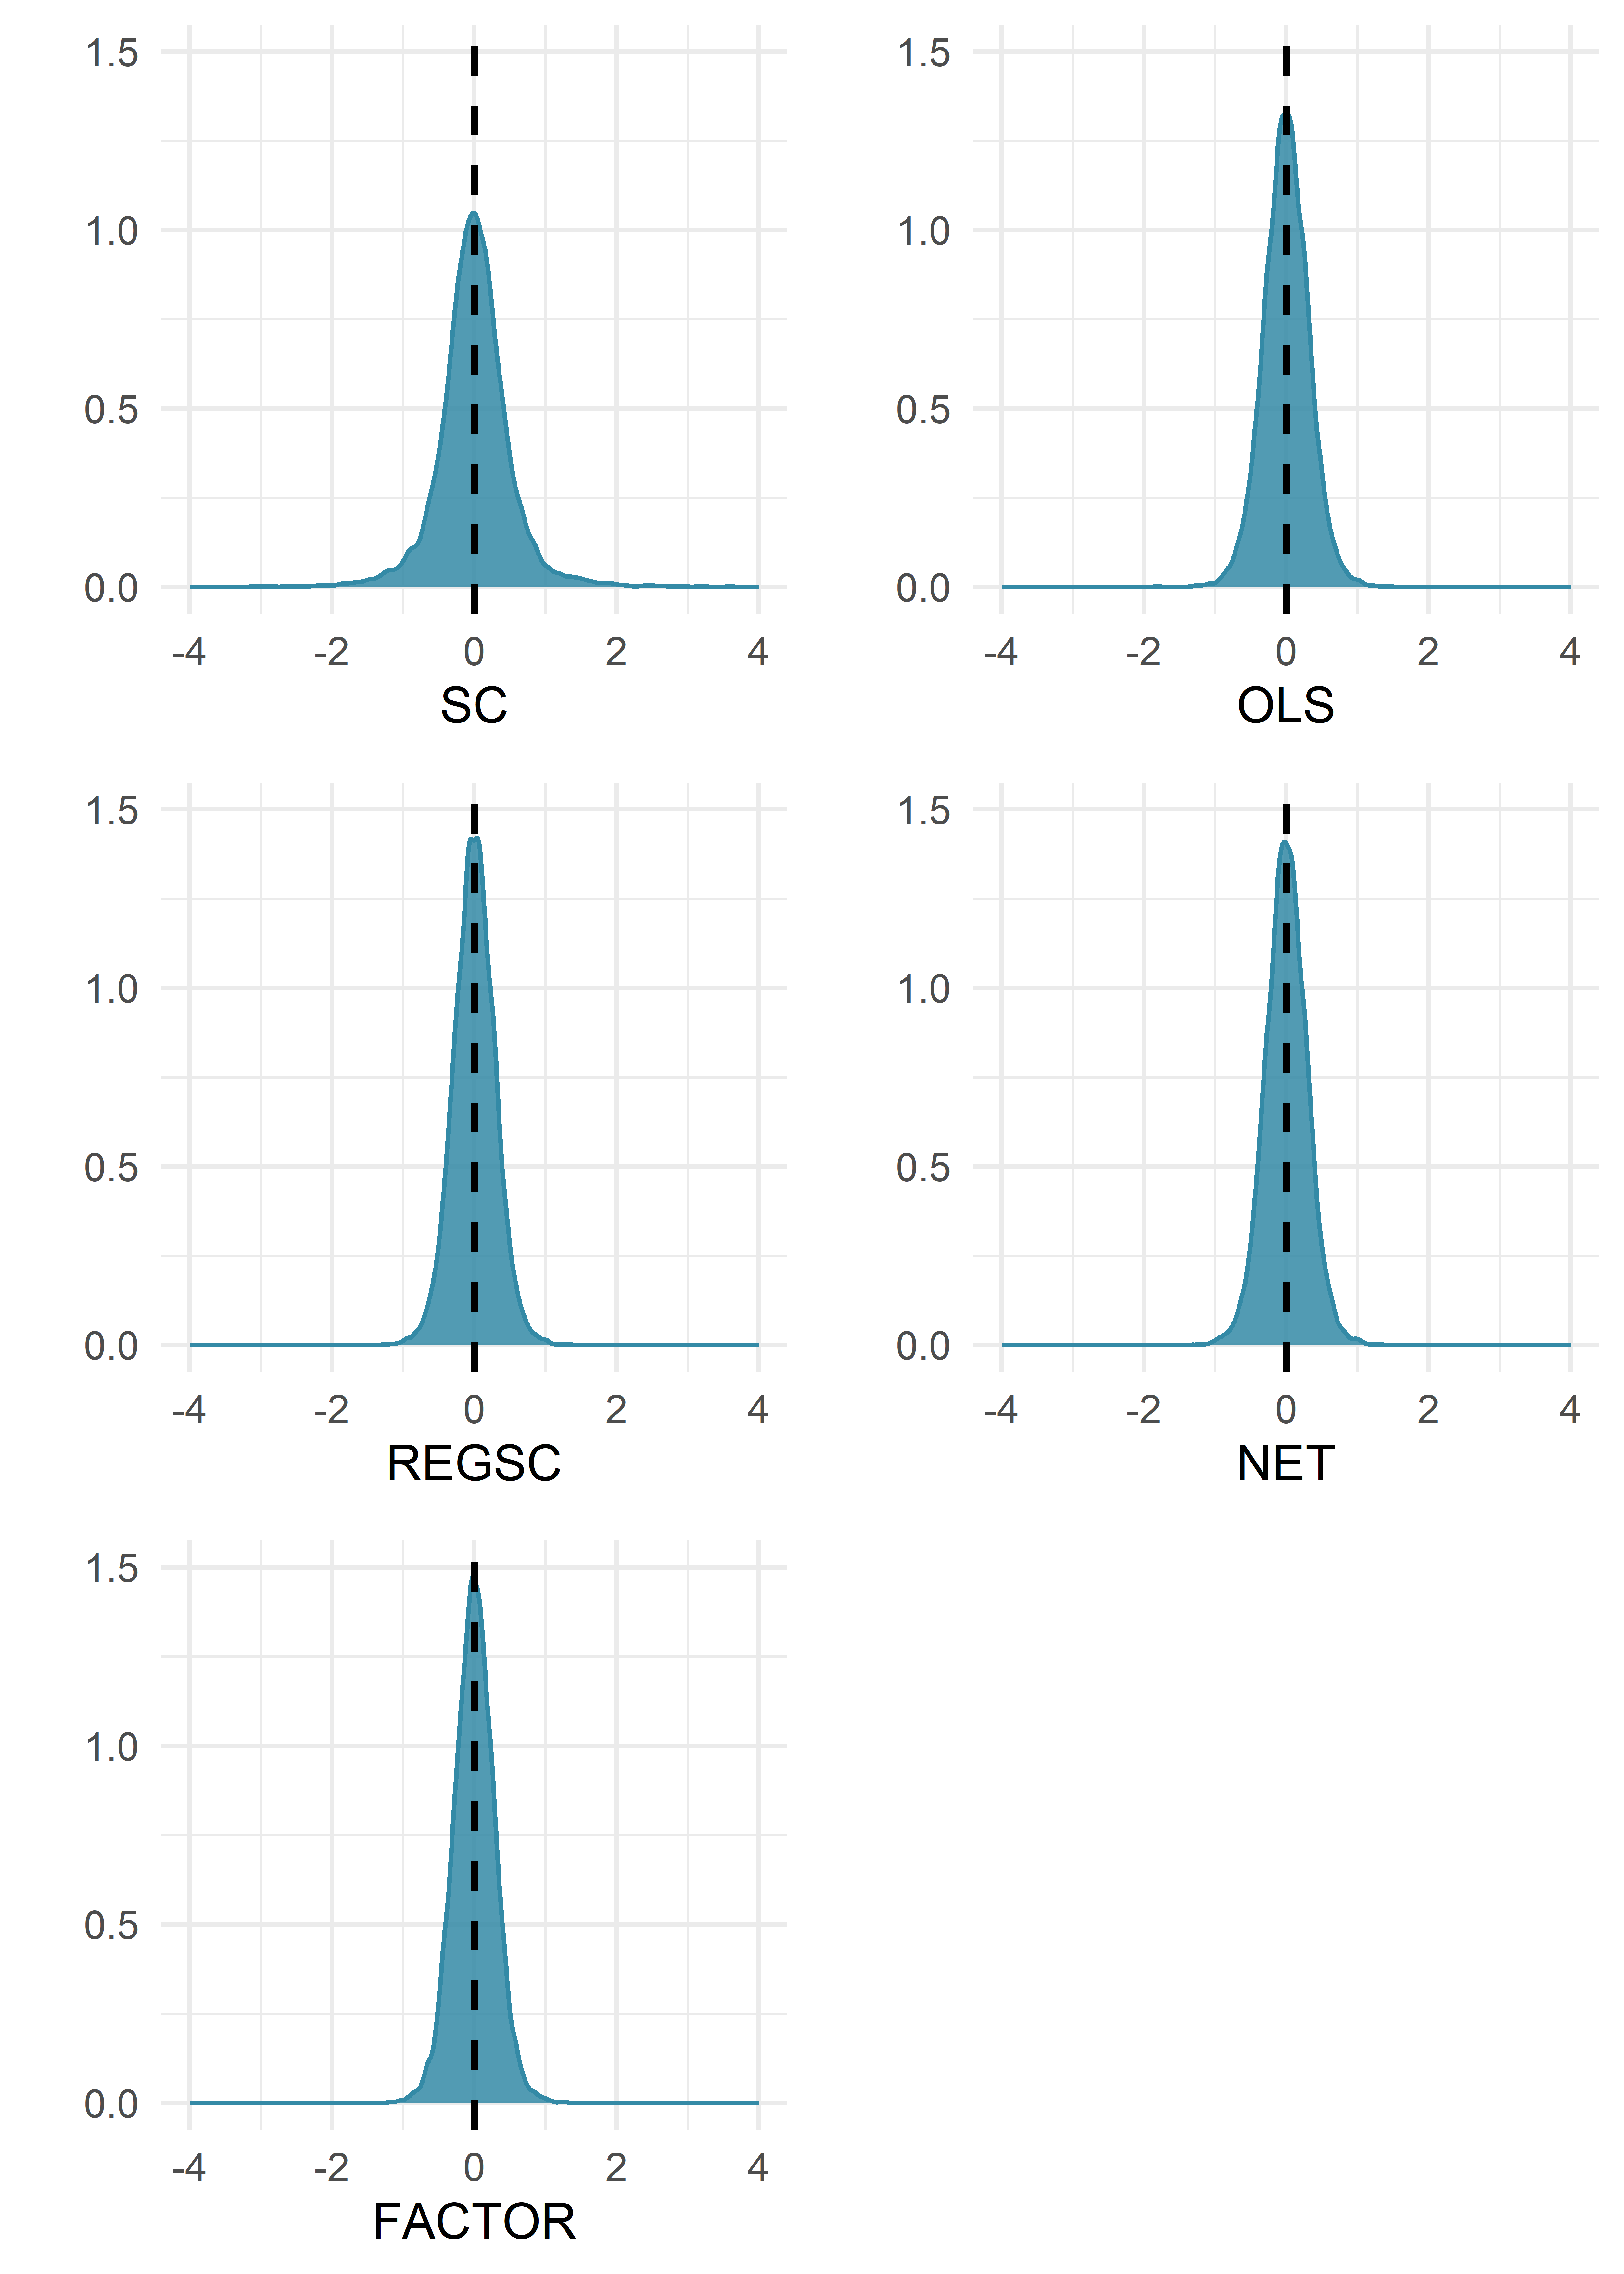
\includegraphics[scale=.9]{F19}
	\caption{Bias-densities for $T_{pre} = 100$ and $T_{post} \in \left\lbrace 10,20,30\right\rbrace$}
	\label{F_14}
\end{figure}

\newpage
\begin{table}[H]
	\centering
	\noindent
	\caption{RMSFE results for $T_{pre} = \in \left\lbrace 20,50,100\right\rbrace$ and $J \in \left\lbrace 5,10,15,20,25,30\right\rbrace$}
	\scalebox{1}{
		\begin{tabular}{c c | C{1.5cm} | C{1.5cm} | C{1.5cm} | C{1.5cm} | C{1.5cm} | C{1.5cm} }
			\toprule[1.5pt]
			\multicolumn{1}{c}{$\boldsymbol{T_{pre}}$} & \multicolumn{1}{c}{\textbf{Donors}}& \multicolumn{1}{c}{\textbf{SC}} & \multicolumn{1}{c}{\textbf{OLS}} & \multicolumn{1}{c}{\textbf{REGSC}}& \multicolumn{1}{c}{\textbf{NET}}& \multicolumn{1}{c}{\textbf{FACTOR}} & \multicolumn{1}{c}{\textbf{2nd best}}\\
			\cmidrule(lr){1-8}
			20&5&1.4438&1.3665&1.2988&1.2980&1.2450&NET\\
			20&10&1.2889&1.6212&1.2294&1.2591&1.1620&REGSC\\
			20&15&1.2444&2.4629&1.2133&1.2377&1.1266&REGSC\\
			20&20&1.2144&NA&1.1961&1.2251&1.1132&REGSC\\
			20&25&NA&NA&1.1976&1.2175&1.1081&REGSC\\
			20&30&NA&NA&1.1724&1.2051&1.0901&REGSC\\
			\cmidrule(lr){1-8}
			50&5&1.4126&1.2101&1.2038&1.1946&1.1735&NET\\
			50&10&1.2366&1.2006&1.1318&1.1404&1.0957&REGSC\\
			50&15&1.1888&1.2640&1.1134&1.1276&1.0740&REGSC\\
			50&20&1.1649&1.3491&1.0999&1.1157&1.0643&REGSC\\
			50&25&1.1515&1.4856&1.0952&1.1104&1.0570&REGSC\\
			50&30&1.1377&1.6422&1.0867&1.1074&1.0474&REGSC\\
			\cmidrule(lr){1-8}
			100&5&1.3886&1.1750&1.1750&1.1689&1.1580&NET\\
			100&10&1.2205&1.1308&1.1044&1.1082&1.0835&REGSC\\
			100&15&1.1695&1.1361&1.0810&1.0879&1.0585&REGSC\\
			100&20&1.1371&1.1575&1.0667&1.0783&1.0443&REGSC\\
			100&25&1.1213&1.1871&1.0580&1.0695&1.0349&REGSC\\
			100&30&1.1105&1.2299&1.0565&1.0704&1.0346&REGSC\\
			\bottomrule[1.5pt]
	\end{tabular}}
	\label{table:table S.8}
\end{table}
	
\end{document}